% Material de borrador: NO se compila.
% Codificación: UTF-8
%
% Contenido antiguo de example.tex que no pertenece a ningún capítulo vigente
% (Introduction, Background, Design and Implementation, Evaluation, Discussion,
% Conclusion). Se conserva aquí como referencia. Este archivo NO se incluye
% desde main.tex; no lo agregues a la compilación sin revisarlo antes.

\chapter{vISA: A small GPU virtual ISA}

This chapter introduces vISA (virtual Instruction Set Architecture), a
simplified and generalized GPU ISA designed to capture the essential
characteristics of modern GPU architectures while being useful for formal
specification and analysis. vISA draws inspiration from contemporary GPU
instruction sets, incorporating key features such as SIMT execution,
hierarchical memory spaces, and a comprehensive instruction set for
general-purpose parallel computing.

\section{Programming model}

vISA provides a single-instruction multiple-thread (SIMT) programming model to
target GPUs that follow this architecture. SIMT architecture is similar to
single-instruction multiple-data (SIMD) model. The key difference is that SIMT
model applies one instruction to independent threads in parallel, instead of
just multiple data lanes. A SIMT instruction controls the execution of a single
thread, whereas SIMD instructions control a vector of multiple data lanes and
exposes the vector width to the software. A SIMT ISA, allows programmers to
write parallel code without dealing with explicit vectors. The SIMT
architecture apply vectorization at runtime rather than at compile-time.

\section{vISA virtual machine}

The vISA virtual machine follows the OpenCL execution model and defines how the
kernels are executed. When the host submits a kernel for execution to the vISA
virtual machine, it defines an N-dimensional index space of up to three
dimensions called the ND-range. When a kernel executes on the vISA virtual
machine, the kernel executes for each element of the ND-range. Each of these
executing kernel functions is called a \textbf{work-item}. The number of total
work-items is known as the global size. Work-items are managed by vISA in
groups called \textbf{work-groups} that cover all the index space. The size of
the work-group is defined by the host program and is known as the local size.
Work-items of the same work-group can communicate through shared memory and
synchronize through barrier instructions. A work-group can be further divided
into subgroups of 32 work-items. Work-items of the same subgroup can
communicate through barrier, shuffle and barrier operations.

The execution of work-groups is concurrent, but not necessarily parallel, and
the execution order is not specified. The work-items of the same work-group are
executed in parallel. Subgroups inside a work-group make independent forward
progress between each other, meaning that execution between them can only be
blocked by synchronization instructions. Inside a subgroup, work items execute
in lockstep fashion, meaning they execute the same instructions simultaneously.
On control flow instructions, when execution diverges, some work-items may be
deactivated, but then be reactivated when control flow re-converges.

\section{Memory Model}
vISA closely follows the OpenCL memory model. vISA work-items may access data
from multiple memory spaces during their execution, as illustrated in Figure
\ref{fig:memory_model}. Each work-item has a private local memory consisting of
registers and private memory space. Each work-group has a shared memory visible
to all work-items of the group with the same lifetime as the work-group.
Finally, all work-items have access to the same global memory, consisting of
the global, constant and parameter memory space.

\begin{figure}[htbp]
    \centering
    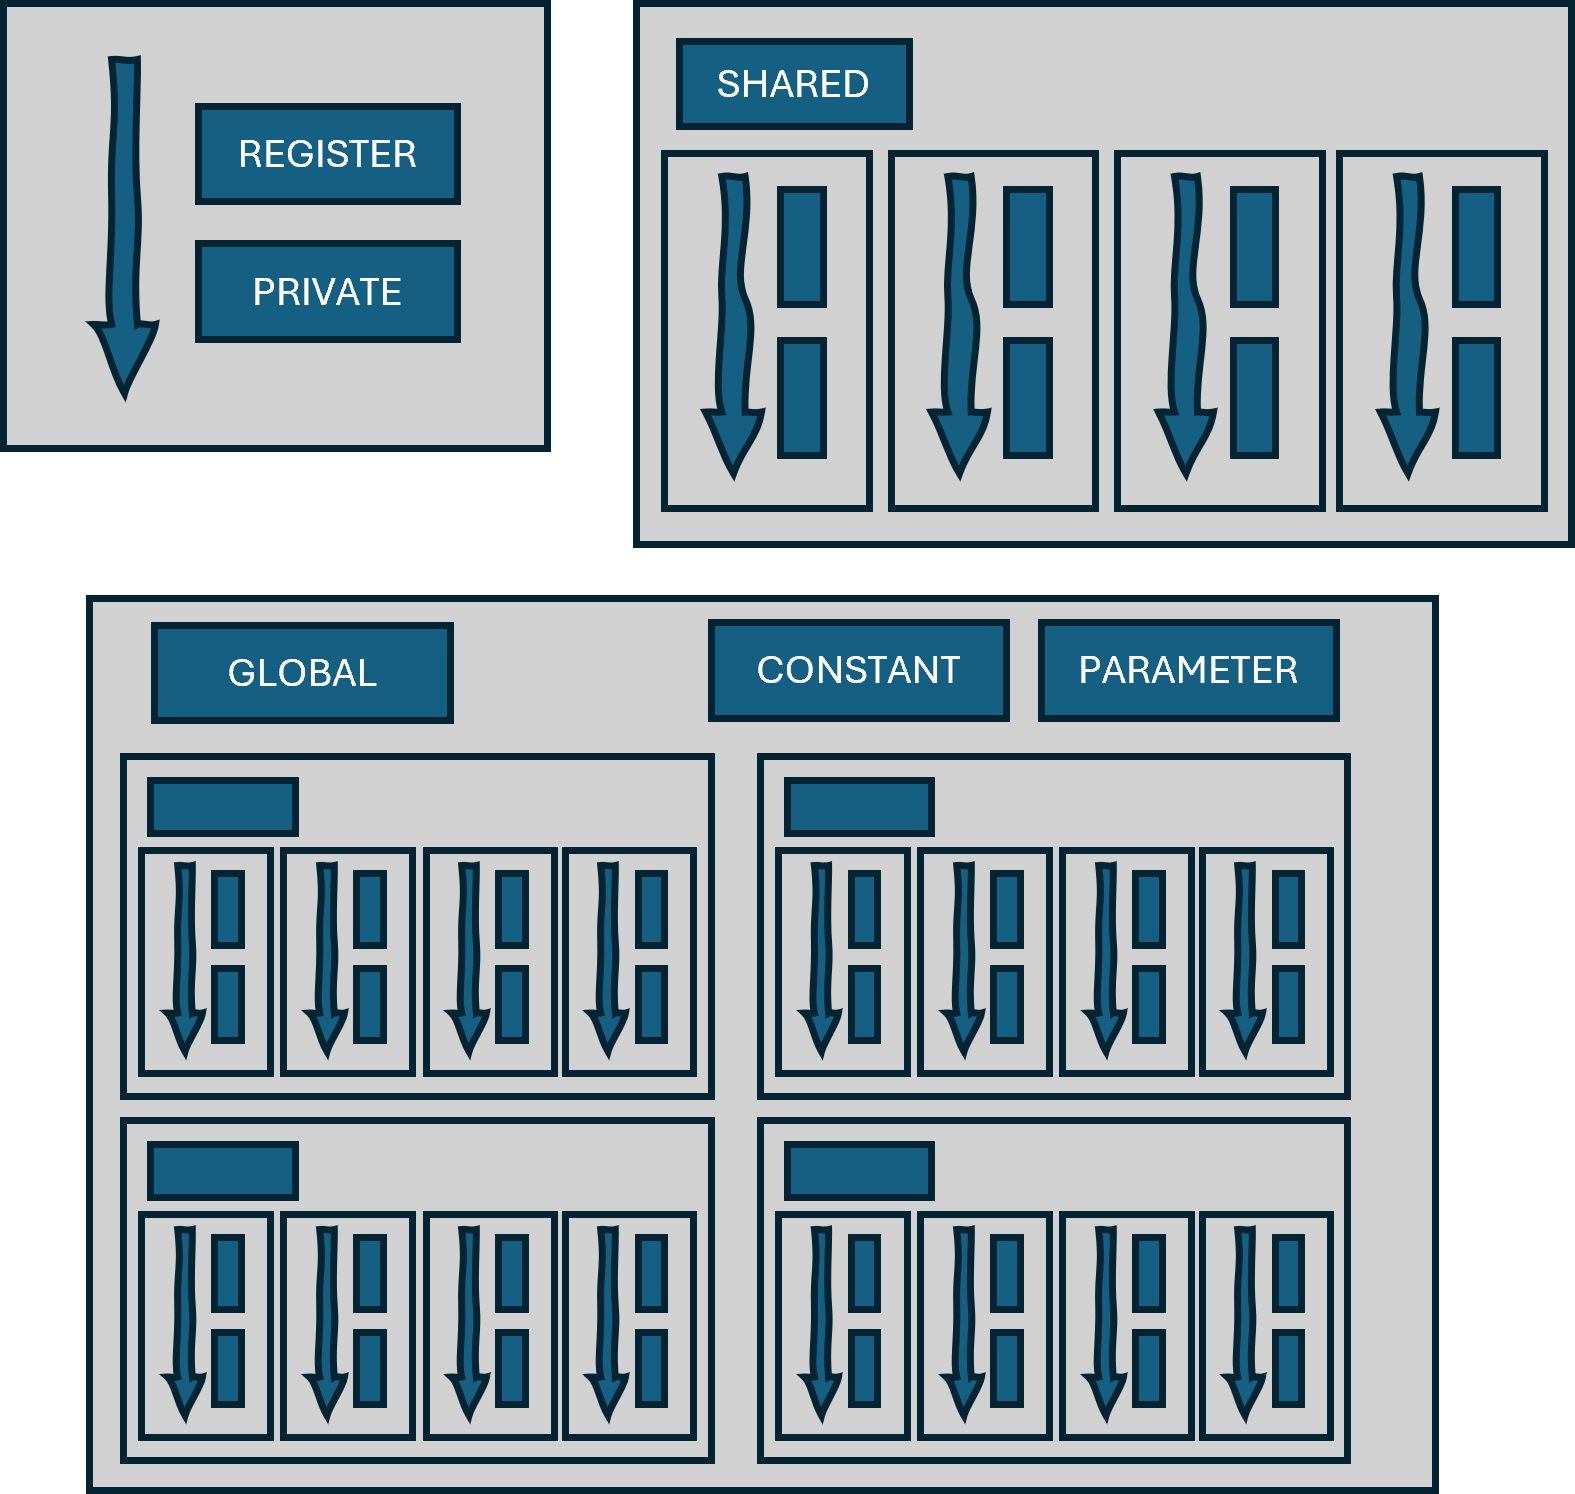
\includegraphics[width=0.6\textwidth]{img/memory.png}
    \caption{vISA memory model}
    \label{fig:memory_model}
\end{figure}

The register space provides high-speed private storage for individual
work-items. Registers can be directly accessed by all vISA instructions without
use of load/store operations. Private memory extends work-item-local storage
beyond register capacity, supporting array objects through explicit
\texttt{load.private} and \texttt{store.private} instructions. Shared memory
enables communication between work-items within the same work-group, providing
read/write access with synchronization support through barrier instructions.
Global memory offers read/write storage accessible by all work-items across the
ND-range, serving as the primary mechanism for host-device data exchange
through \texttt{load.global} and \texttt{store.global} instructions. Constant
memory is read-only and can be accessed by \texttt{load.const} instruction by
all work-items. Parameter memory is read-only and used for for kernel argument
passing from the host program. The global, constant, and parameter memory
spaces are persistent across kernel launches by the same host.

\section{Syntax}

A vISA program is a collection of source text files. vISA files have an
assembly-like syntax, with operation codes (opcode), operands and optional
qualifiers. Inside a vISA file there can be multiple global variable, function
and kernel declarations. Inside the body of functions are kernels are vISA
statements. A statement can be a variable declaration, an instruction or a
label.

\begin{lstlisting}
//variable declaration
.reg .32b %a, %b, %c;
.pred %p;
// label
label:
  // instructions
  sadd.32b   %c, %a, %b;
  store.global.32b  [@A + 16]  %c;
  jump.cond %p label
  
\end{lstlisting}

vISA named identifiers follow some conventions. Kernel, functions and variable
names are prefixed by '@'. Registers are prefixed by '\%'. Labels have no
prefix, but end with ':' character and start a new line.

Instruction syntax starts with their opcode, followed by optional qualifiers,
separated by a dot, and the operands, separated by a comma. In Listing
\ref{lst:instruction_syntax}, '<>' means optional, and '*' zero or more.

\begin{lstlisting}[label={lst:instruction_syntax}]
    opcode.<qualifiers>* <dst>, <src0>, <src1>, <src2>
\end{lstlisting}

\section{Variables}

Variables in vISA have defined bit size and are untyped. This means that data
interpretation is up to the instructions semantics. For example, instruction
\lstinline{sadd.32b} requires destination and source operands to be 32 bits,
and during instruction execution, vISA machine will interpret those values as
signed integer. Supported sizes and types are specified by the instruction
definition. Supported sizes are 8, 16, 32 and 64 bits, and need to be specified
at variable declaration. Supported types are signed and and unsigned integers
of previously mentioned bit sizes and half, bfloat, double and long floating
point types.

Besides regular variables and registers, vISA supports predicates, vectors and
arrays. Predicates and vectors are part of the register space, so they are
private to each work-item. Predicates are used to store the result of
comparison instructions. They are a bit in size, and don't need to specify
their size at declaration. Vectors can have a length of 2, 3 or 4 elements, and
element sizes are as previously specified. Vectors need to specify their length
and element bitsize at declaration. Specific vector elements can be directly
accessed by post-fixing a combination of the component names at the end of the
vector variable name, for example: \lstinline{\%v.x} or \lstinline{\%v.xyzw}.
Finally, arrays can have arbitrary lengths, and are restricted to one
dimension. They can be declared in all memory spaces except register. Supported
element sizes are the default and length of array must be specified at variable
declaration. Listing \ref{lst:variable_declaration} shows examples of the
previously mentioned variable types.

\begin{lstlisting}[label={lst:variable_declaration}]
    .reg .32b %r;
    .reg .v2.32b %v;
    .pred %p;
    .private .32b @A[10];
    .shared .16b @B[10];
\end{lstlisting}

\section{Operands}
vISA instructions accept different operand types. General operands are
variables of the register space, meaning registers, predicates and vectors.
Unless specified otherwise, instructions require that all operands are of the
same bit-width. vISA virtual machine does not handle implicit type conversion
on variables. Any conversion must be done explicitly using conversion
instructions.

Immediate values can be used as sourced operands anywher a scalar operand is
allowed. Immediate values can be in hexadecimal form, prefixed by '0x', or in
decimal form. For type conversion purposes, all immediate values are treated as
64 bit values, hexadecimals are zero-extended and decimals are sign-extended.
When used in instructions, vISA virtual machine converts them to required data
type.

Memory instructions support a special type of operands for address
calculations. Supported address operands are a combination of variables,
registers and immediates. If a variable is used as an address operand, vISA
machine uses the variables byte address in their corresponding memory space.
Meanwhile, registers and immediates are directly interpreted as a byte address.
Address operands also allow direct arithmetic to calculate the address,
allowing an addition between operands. Supported address operands are shown in
Figure \ref{lst:address_operands}.
\begin{lstlisting}[label={lst:address_operands}]
[var + reg]
[var + imm]
[reg + reg]
[reg + imm]
[var]
[reg]
[imm]
\end{lstlisting}

\section{Kernels}
vISA kernels are the entry point of execution and can only be invoked by the
host program. Kernels are named and are defined using the \lstinline{.kernel}
directive. Kernels can have parameters that are initialized by the host
program. Parameters variables exist inside the parameter memory space, they are
prefixed with '\%' and their size is specified in bytes. A parameter can also
be a pointer to memory, in that case, the parameter is decorated with the
\lstinline{.addrspace(ADDRSPACE)} attribute, indicating which memory space it
points to. Parameters can only be used as an address operand, through the
\lstinline{load.param} instruction.

\begin{lstlisting}
.kernel @foo(.param[4] %a, .param[8] .addresspace(global) %b) {
   .reg .32b %local_a;
   .reg .64b %local_b;
   .reg .32b %global_b

// loading parameter value
   load.param.32b %local_a, [%a];
   
// loading 32 bits of global data from pointer parameter
   load.param.64b %local_b, [%b];
   load.global.32b %global_b [%local_b];
}
\end{lstlisting}

\section{Instruction set}
As previously mentioned, vISA offers a SIMT instruction set for general purpose
programming. This means instructions are presented as inherently scalar in
their semantics. An instruction template is what totally describes an
instruction in vISA. Templates present the instruction's opcode, qualifiers if
any, supported bitsizes and operands. It also includes a description of the
instructions behavior, but most importantly, it presents the instructions
semantics in form of C-like pseudo code.

As an example, Figure \ref{fig:scmp} shows the instruction template for the
signed compare instruction. In the syntax section, the general form of the
instruction is presented, along with the possible values for \lstinline{.cond}
and \lstinline{.bitsize}. Description section describes the instruction and
presents some restrictions the instruction has. Finally the semantics section,
shows the semantics of the instruction in pretty straightforwards pseudocode.
Note that the template shows the instruction as scalar.

\begin{figure}[htbp]
    \centering
    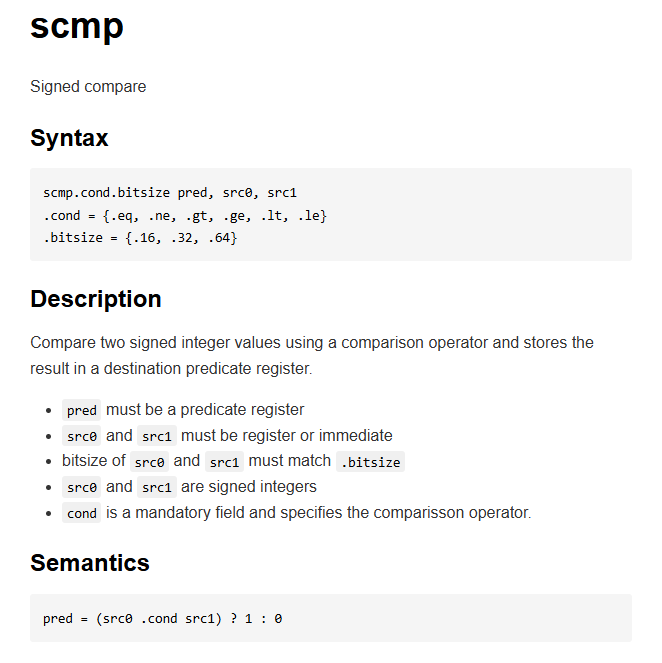
\includegraphics[width=0.8\textwidth]{img/scmp.png}
    \caption{Instruction template for scmp}
    \label{fig:scmp}
\end{figure}

Important instructions in vISA are the control flow instructions as the
\lstinline{jump} instruction shown in Figure \ref{fig:jump}. As previously
mentioned when execution diverges, some work-items are deactivated and then
reactivated. Being a virtual ISA, the exact way that this happens is not
described, since the behavior is implemented by the hardware ISA of the GPU. So
control flow instructions in a virtual ISA do not have much information to the
user in these aspects.

\begin{figure}[htbp]
    \centering
    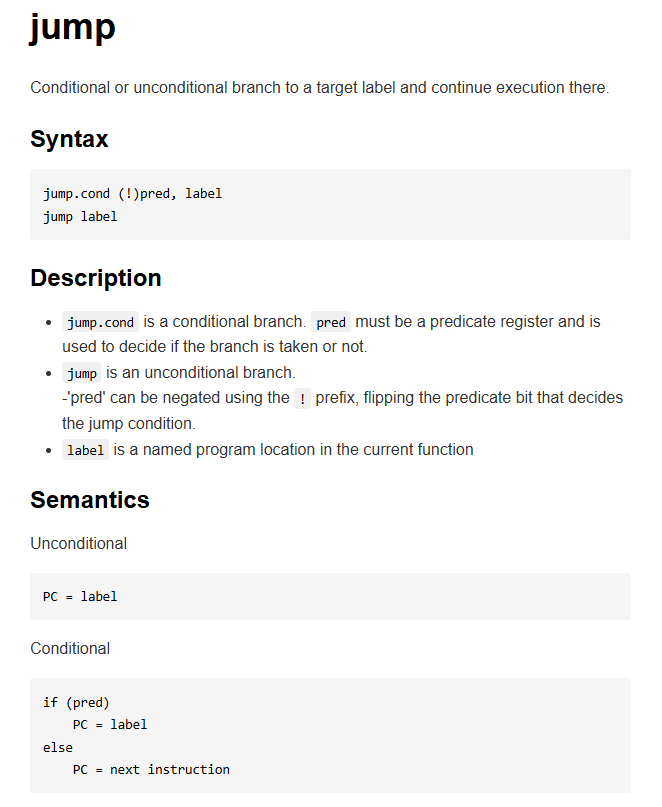
\includegraphics[width=0.8\textwidth]{img/jump.png}
    \caption{Instruction template for jump}
    \label{fig:jump}
\end{figure}


vISA also presents instructions that explicitly describe interaction with other
work-items, exposing the vector nature of the instructions. For example
\lstinline{shfl} instruction excahnge data between the registers of work-items
in a subgroup. The access to other work-items data is explicit in the
instructions semantics, as shown in \ref{fig:shfl}.

\begin{figure}[htbp]
    \centering
    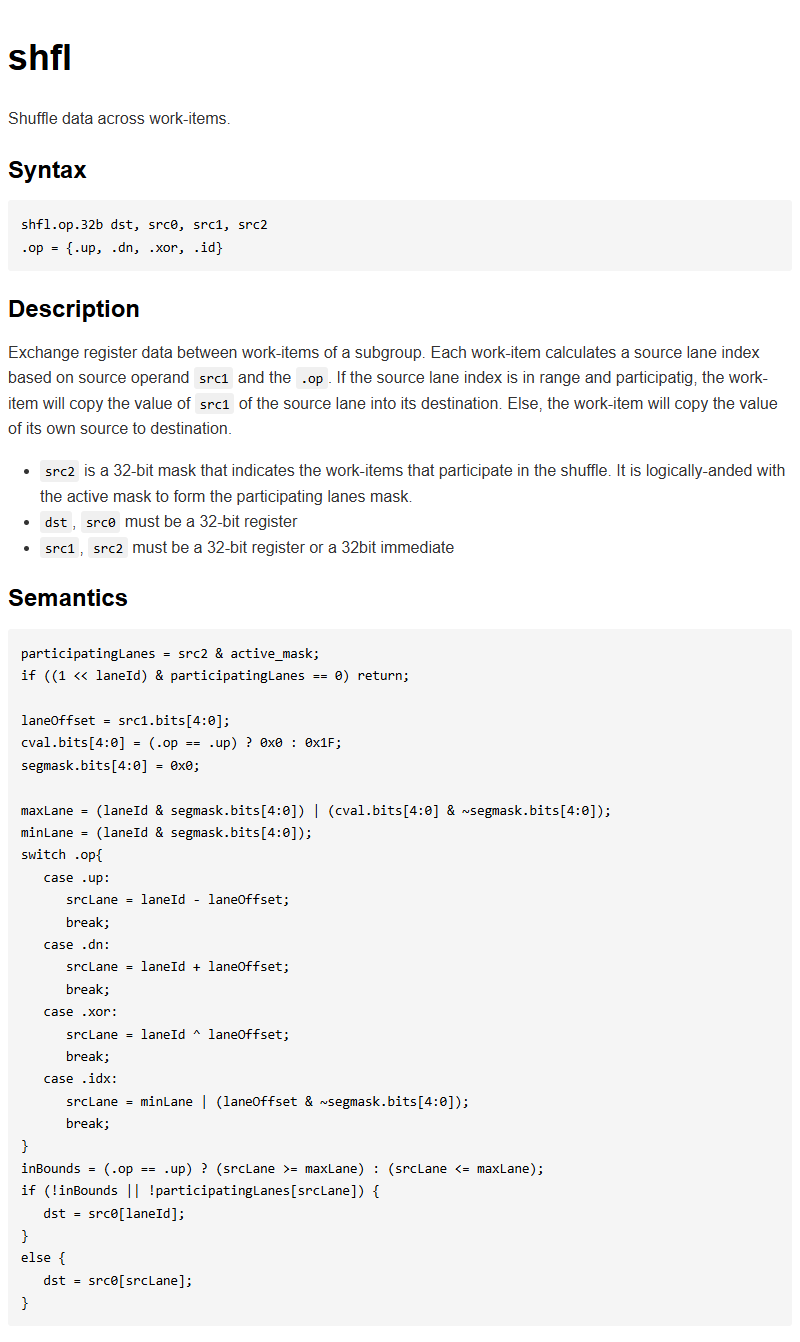
\includegraphics[width=0.8\textwidth]{img/shfl.png}
    \caption{Instruction template for shfl}
    \label{fig:shfl}
\end{figure}

\chapter{Design Overview}
The goal of this thesis is to develop an executable specification of vISA using
Arm’s Architecture Specification Language (ASL). The specification will play
three roles: precise documentation, an executable model, and a testable
reference.

As documentation, the ASL model captures the semantics of vISA at the
instruction level. Each instruction is described in terms of its effect on the
architectural state: registers, control flow, and memory spaces. The
specification is organized so that these semantics are readable and traceable
back to the vISA documentation.

As an executable model, the ASL code can be run to emulate the behaviour of
vISA kernels. A formal state model represents threads, subgroups, and the
different memory regions. The operational semantics define how the state
evolves as each instructions is executed. This makes it possible to step
through vISA programs and observe their effects on the architecture.

To make the specification testable and practically usable, it is integrated
into a toolchain with two additional components: a vISA parser and a custom
OpenCL-based runtime library. The parser translates vISA source code into an
instruction format consumable by the ASL model, while the runtime library sets
up host-side execution (kernels, arguments, and buffers) and invokes the
ASL-based simulator. Together, these components allow vISA kernels to be
executed directly using the specification, enabling systematic testing,
comparison with hardware, and regression checking.

\chapter{Executable vISA specification in ASL}

This chapter covers the design and implementation of the executable vISA
specification written in ASL. It explains how the architectural state is
modeled, how vISA instructions are represented and interpreted, and how SIMT
execution and memory are captured in the model. The purpose of the design
choices is to balance faithfulness to the vISA specification with executability
and practicality.

\section{State Model}
The state model defines the architectural entities that the ASL specification
manipulates during execution. In this work, the state is organized into four
main components: the thread state, subgroup state, memory state, and the global
execution context. We choose this to mirror how vISA structures its execution,
threads are the minimal unit of computation, threads are then grouped into
subgroups, working as the SIMT scheduling and synchronization units, and memory
spaces are defined independently of control. This separation also makes the
specification modular. Most instructions only modify the thread and memory
state, while SIMT- specific behaviour is isolated in the subgroup layer and
global context, like the program and NDRange configuration remains at the top
level.

\subsection{Thread state}

Each vISA thread is represented by a small record containing a program counter,
which indicates the next instruction to execute, and a termination flag, which
records whether the thread has finished execution. All data associated with a
thread is stored in a thread-private region of the memory model. For each
thread, the memory model allocates an isolated segment that holds its virtual
register values, private variables, and special registers (such as thread ID,
subgroup ID, and work-group ID). Instructions access these values indirectly,
by reading and writing the corresponding locations in the thread’s private
memory segment rather than fields in the thread record itself.

\subsection{Subgroup state}
Threads are grouped into subgroups of 32 threads to model vISA's SIMT execution
model, following the OpenCL notion of subgroups. A subgroup is represented as a
fixed array of 32 thread states together with an \emph{active mask} that
indicates which threads are currently participating in execution. In addition,
the subgroup maintains a program counter that indicates the next instruction to
be issued for the active threads.

The active mask is updated by control-flow and predicated instructions to
reflect divergence: when different threads within a subgroup take different
control-flow paths, only the threads for the currently selected path remain
active, while the others are temporarily masked out.

\subsection{Memory state}
The memory state models the different memory spaces exposed by vISA and
provides the storage for all thread-visible data. In the ASL specification,
memory regions are represented using the built-in \lstinline{__RAM} type, which
provides a byte-addressable array with builtin read and write functions.

A design choice in this specification is to store all per-thread data in
dedicated regions of the register memory. For each thread, the memory state
allocates a private segment in a register/private-memory \lstinline{__RAM}
object that serves as its register file and local storage. Virtual registers,
named variables, and architectural special registers are all mapped to fixed
offsets within this private segment.

These private segments are created explicitly during kernel setup. The parser
reads the raw vISA assembly, extracts register and variable declarations at the
start of each kernel, and emits the corresponding ASL allocation functions.
Each allocation call takes the variable identifier, size, memory space, and
calculates the final address in the \lstinline{__RAM} region. At the same time,
the allocation functions populate a \emph{variable map} that records, for each
declared variable, its location in memory. The resulting mapping from vISA
names to offsets is fixed for the lifetime of the kernel, so that instruction
semantics can treat register and variable access as ordinary memory reads and
writes into the corresponding per-thread region.

In addition to these per-thread segments, the memory state includes shared and
global regions that are accessible by multiple threads. Shared memory is
allocated per work-group and is used to model block-level communication and
synchronization, while global memory is visible to all threads in the range and
is used for kernel inputs and outputs.

\subsection{Global state}
The global state ties together the thread, subgroup, and memory components
described above into a single top-level state on which the ASL semantics
operate. Conceptually, it represents the state of a complete kernel launch. It
contains the decoded program to be executed, the grid and work-group
configuration, the collection of subgroups and their associated thread states,
and the memory state with all per-thread, shared, and global regions. In the
ASL specification this is captured by a single record type that is threaded
through all semantic functions, so that each instruction step takes a global
state as input and produces an updated global state as output.

The program component of the context consists of an array of decoded vISA
instructions represented as records. Labels that appear in the source kernel
are resolved by the parser: each label identifier is mapped to the index of the
corresponding instruction in the decoded instruction array, and this
information is stored in a \emph{label map}. During decoding, jump instructions
use this label map to replace label references with instruction addresses, so
that the ASL semantics can perform control-flow changes by modifying program
counters directly.

The range configuration contains the number and dimensions of work-groups and
subgroups, and is used to initialize the subgroup and thread states, along with
their special registers.

The global state is constructed collaboratively by the host code and the
initialization functions introduced by the parser. The host program, using the
custom ASL OpenCL library, setup the range configuration (number of threads and
groups) and allocates and load all input buffers and global memory regions. The
initialization functions install the decoded program and label map into the
context and then binds the kernel’s arguments to the concrete global-memory
locations provided by the host. In particular, it links each arguments declared
in the kernel to the corresponding base address in global memory, so that
parameter loads in the semantics can be implemented as ordinary global-memory
accesses. Once this initial state has setup, execution consists of repeatedly
applying the step semantics to the global state until all threads have ended
execution.

\section{Instruction Representation and Decoding}

In order to execute vISA instructions, they need to be translated from their
text form to an internal representation that the ASL semantics can operate on
directly. This ASL representation contains all the information needed to define
instruction behavior. The transformation from textual vISA to ASL is performed
by the parser described in Chapter X, which also handles the allocation of
variables and resolution of labels as discussed in the previous section.

Each instruction in the ASL representation is captured as a record containing
an opcode that identifies the instruction, a collection of operand descriptors
that specify the sources and destinations, and instruction-specific qualifiers
that define the semantics of each operation. Operand descriptors encode whether
an operand refers to a register, an immediate value, or an address operand, and
they include the necessary identifiers to locate the corresponding data during
execution. For registers and variables, these identifiers are resolved using
the variable map populated during the allocation phase, so that the ASL
semantics can fetch the operand data using their memory addresses without
further name resolution.

The instruction-specific qualifiers capture semantic variations that affect how
each instruction behaves. For example, comparison instructions such as
\lstinline{cmp} include qualifiers that specify the comparison operation to
perform: less-than (\lstinline{lt}), greater-than (\lstinline{gt}), equal
(\lstinline{eq}), less-or-equal (\lstinline{le}), and so forth. Similarly,
memory instructions carry qualifiers that indicate the target address space
(global, shared, local) and any ordering or caching behaviour. During
execution, each instruction's function checks for these qualifiers to determine
the exact operation to perform, allowing a single ASL function can handle
multiple variants of an instruction.

Data type information is inferred from the combination of vISA instruction
bitwidth qualifiers and the semantics of the instruction itself. The bitwidth
qualifier specifies the size of the data being operated on (for example,
16-bit, 32-bit, or 64-bit), while the instruction's semantic class determines
how that data should be interpreted. For example, a \lstinline{fadd}
instruction operating on 32-bit data will interpret its operands as
single-precision floating-point values, while a \lstinline{uadd} instruction
with the same 32-bit qualifier will treat the operands as unsigned integers.
This makes it easier to represent since we only save the bitwidth of the
instruction.

\section{Instruction Semantics}

The operational semantics of vISA instructions are implemented as ASL functions
that define the computational behavior of each instruction type. These
functions abstract the core logic of instruction execution from the
complexities of SIMT coordination and subgroup management, which are handled
separately in the execution framework described in Section 4.4.

\subsection{ASL Function Model}

Instructions in the specification are modeled as pure ASL functions that follow
a consistent signature pattern. In the general case, an instruction function
takes the decoded input data as arguments, along with the instruction record
containing any additional qualifiers needed to determine the precise operation
to perform. The function interprets the input data according to the
instruction's semantics, performs the required computation, and returns a
result value that corresponds to a write to the instruction's destination
operand.

For example, the general form of an instruction function is:
\begin{lstlisting}
function template(bitwidth : integer { 8, 16, 32, 64 }) 
    instruction_name(src0 : bits(64), src1 : bits(64), ..., instruction : Instruction) => bits(64)
\end{lstlisting}

Almost all vISA instructions include a bitwidth qualifier that determines the
size and interpretation of operand data. To handle this systematically,
instruction functions are defined as templates parameterized by bitwidth, with
the template parameter constrained to the set of supported sizes (8, 16, 32,
and 64 bits). This design serves two purposes: it captures the polymorphic
nature of vISA instructions that operate on multiple data sizes, and it
provides ASL with the explicit type information needed to resolve polymorphism
when translating the specification to C. Without the template parameter, ASL
cannot determine which concrete types to generate for \lstinline{bits(N)}
operations during compilation.

The input operands are provided as the raw bit data rather than symbolic
references, having been resolved during the operand decoding phase. All
operands are represented uniformly as 64-bit values, with the actual
interpretation determined by the bitwidth parameter and the instruction's
semantic class. The instruction record provides access to qualifiers that
affect the operation's behavior, such as comparison types for conditional
instructions, address spaces for memory operations, or signed/unsigned
interpretation flags that work together with the bitwidth to determine complete
data semantics.

Most instruction functions follow a purely functional approach with no direct
state mutation: they compute and return a result value, and the writes to the
destination registers are handled by the execution framework. However, certain
special instructions such as jumps, and synchronization operations do perform
state mutations as part of their semantics, since their primary purpose is to
affect control flow or inter-thread coordination rather than to produce data
values. In these cases, the state modifications are made explicit in the
function definition to maintain clarity about the instruction's effects.

\subsection{From vISA to ASL: Instruction Representation Examples}

To illustrate how vISA instructions are translated into executable ASL
semantics, this section presents several representative examples that
demonstrate the mapping from textual instruction syntax to functional
specification code.

\subsubsection{Arithmetic Instruction Example}

Consider the vISA integer addition instruction:
\begin{lstlisting}
add.s32 %r1, %r2, %r3
\end{lstlisting}

This instruction adds two signed 32-bit integers and stores the result. In the
ASL specification, this is represented as:

\begin{lstlisting}
function execute_add(src1: bits(32), src2: bits(32), instr: InstructionRecord) => bits(32)
begin
  let bitwidth = instr.bitwidth_qualifier;
  let is_signed = instr.opcode == ADD_SIGNED;
  
  case bitwidth of
    when 32 => 
      if is_signed then
        return src1 + src2;  // Signed 32-bit addition
      else
        return src1 +_u src2;  // Unsigned 32-bit addition
    when 64 => 
      // Handle 64-bit variants...
  esac;
end
\end{lstlisting}

The vISA textual instruction carries its semantics through the opcode (`add`)
and type qualifier (`.s32`), which specify signed 32-bit integer arithmetic.
The ASL function receives the resolved operand values (`src1`, `src2`) and uses
the instruction record to determine the precise operation variant. The type
qualifier guides both the bit width and the arithmetic interpretation, ensuring
that the specification faithfully reproduces the vISA semantics while remaining
executable.

\subsubsection{Memory Instruction Example}

A global memory load instruction illustrates how address computation and memory
space selection are handled:
\begin{lstlisting}
ld.global.f32 %r1, [%r2 + 16]
\end{lstlisting}

This instruction loads a 32-bit floating-point value from global memory at the
address computed by adding an offset to a base register. The corresponding ASL
function is:

\begin{lstlisting}[language=ASL]
function execute_load(base_addr: bits(64), offset: integer, instr: InstructionRecord) => bits(32)
begin
  let effective_addr = base_addr + offset;
  let memory_space = instr.address_space_qualifier;
  let data_type = instr.type_qualifier;
  
  case memory_space of
    when GLOBAL => 
      case data_type of
        when FLOAT32 => return load_global_f32(effective_addr);
        when UINT32 => return load_global_u32(effective_addr);
        // Other type variants...
      esac;
    when SHARED => 
      // Handle shared memory access...
    // Other address space variants...
  esac;
end
\end{lstlisting}

The ASL function captures the address computation logic (base + offset) and
uses the instruction qualifiers to select both the appropriate memory region
(global memory) and the correct data interpretation (32-bit floating-point).
The function delegates the actual memory access to helper functions like
\lstinline{load_global_f32} that interact with the global memory
\lstinline{__RAM} object, maintaining the separation between instruction logic
and memory system implementation.

\subsubsection{Control-Flow Instruction Example}

Predicated branch instructions demonstrate how control-flow and conditional
execution are handled:
\begin{lstlisting}
@p1 bra target_label
\end{lstlisting}

This instruction branches to a target label if predicate register
\lstinline{p1} is true. Unlike data-producing instructions, branches directly
modify the execution state:

\begin{lstlisting}[language=ASL]
function execute_branch(predicate_val: boolean, target_pc: integer, 
                       thread_state: ThreadState, instr: InstructionRecord) => ThreadState
begin
  if predicate_val then
    return thread_state with { pc = target_pc };
  else
    return thread_state with { pc = thread_state.pc + 1 };
  endif;
end
\end{lstlisting}

This function exemplifies the explicit state mutation mentioned earlier:
instead of returning a data value, it returns an updated thread state with a
modified program counter. The target address is provided as a resolved
instruction index (computed from the label map during decoding), and the
predicate value is evaluated from the thread's current predicate register
state.

\subsection{ASL Features for Documentation and Executability}

The ASL specification serves dual purposes as both executable code and readable
documentation. Several language features support this goal. Pattern matching
and case analysis make the specification's decision logic explicit and easy to
follow. Type annotations clarify the data formats expected by each function,
while the functional programming style mirrors the mathematical precision
typical of formal specifications. Built-in ASL constructs like the
\lstinline{__RAM} type provide hardware-realistic abstractions without
requiring low-level implementation details, allowing the specification to focus
on architectural semantics rather than system-level concerns.

The resulting ASL code functions as executable pseudocode that can be directly
compiled and run while remaining sufficiently high-level and structured to
serve as authoritative documentation of the vISA instruction semantics. This
approach ensures consistency between the specification and its implementation,
since they are literally the same artifact.

\section{SIMT Execution and Scheduling}

The vISA follows the SIMT execution model (Single Instruction, Multiple
Thread), where thread subgroups are executed in lockstep. While individual
instruction semantics define the computational behavior of each operation, the
SIMT execution framework coordinates how these semantics are applied across
multiple threads, handles divergence when threads take different control paths,
and manages synchronization between threads within a work-group.

\subsection{Execution Model Overview}

The execution of vISA programs follows a structured pipeline that operates on
subgroups of 32 threads. For each execution step, the framework selects an
eligible subgroup and processes it through four main phases: instruction fetch,
operand decoding, instruction dispatch, and result writeback. This pipeline is
applied to all active threads in the selected subgroup, maintaining the
appearance of concurrent execution while actually processing threads
sequentially due to the constraints of the ASL specification framework.

Instruction fetch retrieves the instruction pointed to by the subgroup's
program counter from the decoded instruction array stored in the global
execution context. All active threads in a subgroup share the same program
counter and therefore execute the same instruction in lockstep. The fetch phase
simply retrieves the single instruction that all active threads will execute.

The operand decoding phase is common across many instruction types and handles
the resolution of operand descriptors to concrete data values. For each thread,
register and variable operands are fetched from the thread's private memory
segment using the variable map established during initialization. Immediate
operands are extracted directly from the instruction record. This phase
produces the concrete operand values that will be passed to the
instruction-specific semantic functions.

Instruction dispatch calls the appropriate ASL semantic function for the
instruction fetched in the current step. The semantic function receives the
decoded operand values, the bitwidth template parameter, and the instruction
record, and computes the results according to the instruction semantics defined
in Section 4.3. Since all active threads execute the same instruction, only one
semantic function is invoked per subgroup step, but it is applied to the
operand values from each active thread.

Result writeback stores the computed results in the appropriate destination
locations. For most instructions, this involves writing to register or variable
locations in each thread's private memory segment. Control-flow instructions
may update the subgroup's shared program counter or modify the subgroup's
active mask instead of producing data results. Instructions with side effects,
such as memory stores or barrier operations, apply their effects to the shared
architectural state.

\subsection{Subgroup Scheduling and Active Masks}

The SIMT execution framework maintains an active mask for each subgroup that
indicates which threads are currently participating in execution. Threads
become inactive when they are disabled by predication, when they have reached a
barrier and are waiting for other threads, or when they have terminated. Only
active threads participate in instruction execution, though inactive threads
maintain their architectural state and may become active again later. All
active threads in a subgroup share a common program counter that determines
which instruction the subgroup will execute next.

Subgroup scheduling determines which subgroup to execute in each step of the
simulation. For ease of execution, the specification makes a design decision to
limit work-group size to 32 threads, the same as subgroup size, meaning each
work-group contains exactly one subgroup. Subgroups are dispatched sequentially
in a simple incremental order, skipping any subgroups that have no active
threads or are blocked waiting for synchronization. This scheduling policy
ensures forward progress and deterministic execution, though it does not
attempt to model the complex scheduling behaviors of real GPU hardware.

When control-flow instructions cause threads within a subgroup to take
different paths, the active mask is updated to reflect the current execution
state. Threads that take a branch have their active status determined by the
branch condition and the subgroup's execution strategy. The specification
implements a simplified divergence model where the subgroup maintains separate
execution contexts for different control-flow paths.



\section{Control-Flow Divergence and Reconvergence}

The specification implements a lockstep SIMT execution model that manages
thread divergence through explicit program counter management and thread
activation/deactivation mechanisms. A key constraint in modeling vISA is that
the instruction set does not include explicit instructions for reconvergence.
Unlike some GPU architectures that provide compiler-inserted reconvergence
annotations, vISA requires a method that can reconverge threads implicitly
based on control-flow analysis alone.

To address this requirement, the specification adopts the stack-less, implicit
reconvergence approach presented in "Stack-less SIMT reconvergence at low cost"
[CITE]. This paper proposes a correct method for implicit reconvergence that
operates without maintaining auxiliary stack structures or requiring explicit
reconvergence markers in the instruction stream. The approach has been formally
analyzed and proven correct, making it an ideal foundation for an executable
specification. This is a deliberate design choice and does not represent any
specific real hardware behavior, as vISA is a virtual instruction set that may
be implemented differently across various platforms.

Stack-less and implicit reconvergence techniques have been explored separately
in various processor architectures. Intel's Sandy Bridge integrated GPU
maintains individual program counters per thread without stack structures
[CITE], while other architectures have implemented implicit reconvergence
without compiler annotations [CITE]. The approach adopted here follows the
algorithms presented in the stack-less reconvergence paper.

\subsection{Divergence and Reconvergence Algorithms}

In this model, each thread maintains an individual program counter $PC_i$ that
independently tracks its position in the instruction sequence. A global program
counter $PC_{global}$ determines which instruction the subgroup will execute
next, and an execution mask $M$ indicates which threads are currently active.
For the general case of instructions that do not cause divergence, all active
threads have their individual program counters incremented in lockstep: $PC_i
\leftarrow PC_i + 1$ for all $i$ where $M[i] = 1$, and the global program
counter advances similarly: $PC_{global} \leftarrow PC_{global} + 1$.

The fundamental reconvergence condition is:

$$\text{Thread } i \text{ is reactivated when } PC_i = PC_{global} \text{ and } M[i] = 0$$

Figure~\ref{fig:divergence_execution} illustrates the execution flow of four
threads through a sequence of jump instructions. Each execution step shows the
state of the execution mask (colored squares indicate active threads) and the
individual thread program counters. The figure demonstrates how threads diverge
at conditional branches and automatically reconverge when their program
counters align with the global program counter.

The divergence handling algorithm distinguishes between forward and backward
jumps based on the relationship between the jump target $PC_{target}$ and the
current global program counter. Figure~\ref{fig:jump_cases} formalizes the two
cases:

\textbf{Forward Jump Algorithm} ($PC_{target} > PC_{global}$):
\begin{itemize}
    \item For each thread $i$ that takes the jump: $PC_i
    \leftarrow PC_{target}$, $M[i] \leftarrow 0$
    \item For each thread $i$ that does not jump: $PC_i \leftarrow PC_{global} + 1$
    \item Update global program counter: $PC_{global} \leftarrow PC_{global} + 1$
\end{itemize}

\textbf{Backward Jump Algorithm} ($PC_{target} < PC_{global}$):
\begin{itemize}
    \item For each thread $i$ that takes the jump: $PC_i
    \leftarrow PC_{target}$, $M[i] \leftarrow 1$
    \item For each thread $i$ that does not jump: $PC_i \leftarrow PC_{global}
    + 1$, $M[i] \leftarrow 0$
    \item Update global program counter: $PC_{global} \leftarrow PC_{target}$
    \item Update execution mask to include only jumping threads
\end{itemize}

The asymmetry between forward and backward jump handling is crucial for
correctness. In forward jumps, the global program counter advances
incrementally, guaranteeing that it will eventually reach the target where
deactivated threads wait. In backward jumps, the global program counter
immediately moves to the target to allow looping threads to continue their
iterations, while non-jumping threads are deactivated and wait at subsequent
program points. This asymmetry ensures both progress and eventual reconvergence
without requiring auxiliary data structures.

This divergence and reconvergence algorithm is made explicit in the ASL jump
instruction implementation as an interpretation of its semantics. The jump
instruction processes all threads in the subgroup, evaluates predicates for
conditional jumps, classifies the jump as forward or backward based on the
relationship between the target and current global program counter, and applies
the appropriate algorithm to update thread program counters and the execution
mask. While this explicit handling does not mirror specific GPU hardware
implementations, it faithfully implements the stack-less reconvergence
algorithm to provide correct SIMT execution semantics for vISA.

\chapter{vISA Parser and Translation Tool}

To validate the ASL specification against real vISA code, we developed a
translation tool that converts vISA kernels into executable ASL code. The tool
eliminates the need for manual translation, which would be time-consuming and
error-prone. It is implemented in OCaml, using Ocamllex for lexical analysis
and Menhir for parsing. The tool is limited to strictly translating kernels; it
does not function as a host device and does not set up kernel host code or
parameter values. Kernels without parameters and with a single group of 32
threads can be executed directly after translation.

\section{Translation Example}

Listing~\ref{lst:visa_kernel_example} shows a small vISA kernel with divergent
execution. The kernel takes different paths based on the work-item's local ID.
If \lstinline{localid % 4 == 0}, it calculates the ID value decreased by 1;
otherwise, it doubles it.

\begin{lstlisting}[caption={Example vISA kernel with divergent control flow}, label={lst:visa_kernel_example}]
.kernel  @test()
{
    .reg .32b %r0, %r1, %r2;
    .pred %p0;
    
    and.32b     %r0, %localid.x, 3;
    ucmp.ne.32b %p0, %r0, 0;
    goto.cond !%p0, LBB0_1;
    iadd.32b    %r1, %localid.x, -1;
    goto LBB0_3;
LBB0_1:                                
    iadd.32b    %r1, %localid.x, %localid.x;
LBB0_3:                                 
    mov.32b     %r2, %r1;
    return;
}
\end{lstlisting}

The tool translates this kernel into ASL code that sets up the kernel for
execution in the specification. Listing~\ref{lst:asl_generated} shows the
generated output. The tool handles kernel initialization using standard
predefined procedures: it resets the GPU state, defines the kernel grid size,
and initializes special registers. It detects register and variable
declarations and generates the corresponding ASL allocation functions. Each
instruction is encoded into the instruction buffer with all necessary
information for execution. Labels are both encoded into the buffer and recorded
in the label environment, allowing jumps to their exact position at runtime.

\begin{lstlisting}[caption={Generated ASL code for kernel setup and encoding}, label={lst:asl_generated}]
// Kernel setup
Reset();
SetupKernel(32, 1);
SetupSpecialRegisters();

// Register allocation
Register("%r0", 0, 32);
Register("%r1", 1, 32);
Register("%r2", 2, 32);
Pred("%p0", 3);

// Instruction encoding
InstructionBuffer[0].opcode = and;
InstructionBuffer[0].inst_type = BitwiseInst;
InstructionBuffer[0].bitwidth = 32;
InstructionBuffer[0].dst = 0;
InstructionBuffer[0].src0 = SPECIAL_LOCALID_X;
InstructionBuffer[0].use_imm1 = TRUE;
InstructionBuffer[0].imm1 = 3;
...
// Label encoding
SetLabel("LBB0_1", 0, 5);
InstructionBuffer[5].opcode = label;
InstructionBuffer[5].label = 0;
...
\end{lstlisting}

\section{Tool Architecture}

The translation tool follows a standard compiler pipeline with several distinct
stages. The process begins with lexical analysis, where the input vISA code is
tokenized based on terminal symbols defined in the vISA grammar. The parser
then constructs an Abstract Syntax Tree (AST) representing the kernel's
structure, including declarations, instructions, and control-flow elements.
This vISA AST is then transformed into an ASL specification AST, which
represents the setup, allocation, and encoding operations required by the
specification. Finally, the ASL AST is traversed to generate the executable ASL
code.

A critical aspect of the transformation is the management of variable and label
namespaces through two separate mapping structures. During the transformation
from vISA AST to ASL AST, all variable declarations are traversed first, and
each variable is assigned a unique numeric identifier in the variable map. The
identifier counter increments with each new variable added. Labels are handled
during instruction traversal: when the tool encounters either an explicit label
definition or a jump instruction referencing a label, it adds the label to the
label map with a unique identifier if not already present. Variable and label
identifiers exist in separate namespaces, meaning both can independently use
the same numeric values without conflict.

During code generation, when the ASL AST is printed, these maps enable the
translation of textual references to numeric identifiers. Allocation functions
receive both the original string name (for debugging and traceability) and the
assigned numeric ID. Throughout the generated code, all references to variables
and labels use their numeric identifiers rather than string names. Label
positions in the instruction buffer are resolved during this code generation
phase as the tool traverses the instruction list sequentially, determining the
exact buffer index for each instruction and label.

The tool represents kernels using two intermediate ASTs. The vISA AST captures
the parsed structure with types for kernel definitions, variable declarations
(registers, vectors, predicates), instructions (opcodes, qualifiers, operands),
and labels. The ASL AST represents the target operations: kernel parameter
setup, variable allocation calls, and instruction field assignments for buffer
encoding. This separation of concerns allows the transformation logic to focus
on semantic translation while keeping the code generation phase
straightforward.

\section{Summary}

The vISA-ASL translation tool provides an automated mechanism for converting
vISA kernels into executable ASL specification code. By implementing a
systematic parsing and transformation approach with efficient numeric
identifier mapping, the tool eliminates manual translation efforts and enables
systematic validation of the ASL specification against real GPU programs. The
tool bridges the gap between vISA source code and the executable specification,
offering developers a practical method to test existing kernels within the ASL
framework without requiring deep knowledge of the specification's internal
representation.



\chapter{OpenCL ASL Library}

\section{Introduction}

OpenCL (Open Computing Language) is an open standard for parallel programming
across heterogeneous platforms, including CPUs, GPUs, and other accelerators.
It defines a host-device programming model where a host program manages device
resources, transfers data, and enqueues computational kernels for execution on
parallel devices. To facilitate testing and validation of the ASL specification
using familiar parallel programming patterns, we developed a custom OpenCL ASL
library that provides an OpenCL-compatible API while executing kernels on the
ASL specification rather than physical GPU hardware.

The ASL OpenCL library serves as a replacement for the standard OpenCL runtime,
offering host-side programs a familiar interface for interacting with the
executable specification. This approach allows developers to write standard
host code that would normally target GPU hardware, but instead executes against
the ASL model, enabling systematic testing and validation of the
specification's behavior.

\section{OpenCL Programming Model}

The OpenCL programming model revolves around several key concepts and a
well-defined execution flow. A typical OpenCL program operates with platforms
(vendor implementations), devices (computational units), contexts (execution
environments), command queues (task submission mechanisms), memory buffers
(data storage), and kernels (parallel functions).

The standard flow of an OpenCL host program follows these steps:

\begin{enumerate}
    \item \textbf{Platform and device discovery}: Query available OpenCL
    platforms and select appropriate devices using functions like
    \texttt{clGetPlatformIDs} and \texttt{clGetDeviceIDs}
    \item \textbf{Context and command queue creation}: Create an execution
    context and command queue with \texttt{clCreateContext} and
    \texttt{clCreateCommandQueue}
    \item \textbf{Buffer allocation and data transfer}: Allocate device memory
    buffers using \texttt{clCreateBuffer} and transfer data from host to device
    using \texttt{clEnqueueWriteBuffer}
    \item \textbf{Kernel loading and compilation}: Load kernel source code and
    compile it for the target device using \texttt{clCreateProgramWithSource}
    and \texttt{clBuildProgram}, then create kernel objects with
    \texttt{clCreateKernel}
    \item \textbf{Setting kernel arguments}: Bind buffer objects and scalar
    values to kernel parameters using \texttt{clSetKernelArg}
    \item \textbf{Kernel execution}: Enqueue the kernel for execution with
    specified work dimensions using \texttt{clEnqueueNDRangeKernel}
    \item \textbf{Result retrieval}: Transfer results back from device to host
    using \texttt{clEnqueueReadBuffer} and clean up resources
\end{enumerate}

\section{ASL OpenCL Library Implementation}

The ASL OpenCL library is implemented in C++ and imports the C code generated
from the ASL specification. It implements a functional subset of the OpenCL
API, providing the necessary functions to support the execution flow described
above while targeting the ASL specification as the execution backend.

Platform, device, context, and command queue setup functions
(\texttt{clGetPlatformIDs}, \texttt{clGetDeviceIDs}, \texttt{clCreateContext},
\texttt{clCreateCommandQueue}) are implemented as stub functions that provide
API compatibility but perform minimal operations. Since the library targets a
single "device" (the ASL specification), these functions are hardcoded to
return success and provide placeholder handles without complex initialization
logic.

Buffer allocation and data transfer functions are fully implemented and
critical to the library's functionality. The \texttt{clCreateBuffer} function
allocates regions in the ASL specification's global memory \lstinline{__RAM},
reserving space for kernel input and output data. The
\texttt{clEnqueueWriteBuffer} function transfers data from host memory into
these allocated ASL global memory regions, populating them with initial values
before kernel execution. Similarly, \texttt{clEnqueueReadBuffer} retrieves
results from ASL global memory back to host memory after kernel execution
completes.

Setting kernel arguments through \texttt{clSetKernelArg} is essential for
binding host-allocated buffers to kernel parameters. This function establishes
the mapping between OpenCL buffer objects and the kernel's formal parameters,
ensuring that when the kernel executes, its parameter references correctly
point to the corresponding global memory regions in the ASL specification. The
implementation records these bindings so they can be applied during kernel inv



\chapter{Design and Implementation}

As explained in Section x, the main objective of this thesis is to develop an
executable specification for vISA. The specification must serve as
documentation, be executable and testable. For documentation, the specification
must accurately describe the instructions semantics in form of ASL code. It
must be able to execute the instructions and emulate their effect on memory and
architecture. Lastly, it must be testable, meaning the specification must be
able to easily execute vISA code and provide results.

Our solution consists of two parts: the actual specification for the vISA
virtual machine written in ASL, and a complementary translation tool, that
parses and loads vISA workloads into the virtual machine.

A general diagram of the design of the specification is shown in Figure X. The
proposed and implemented specification for the virtual machine has two main
parts: the machine state, and the machine behavior.

\begin{figure}[htbp]
    \centering
    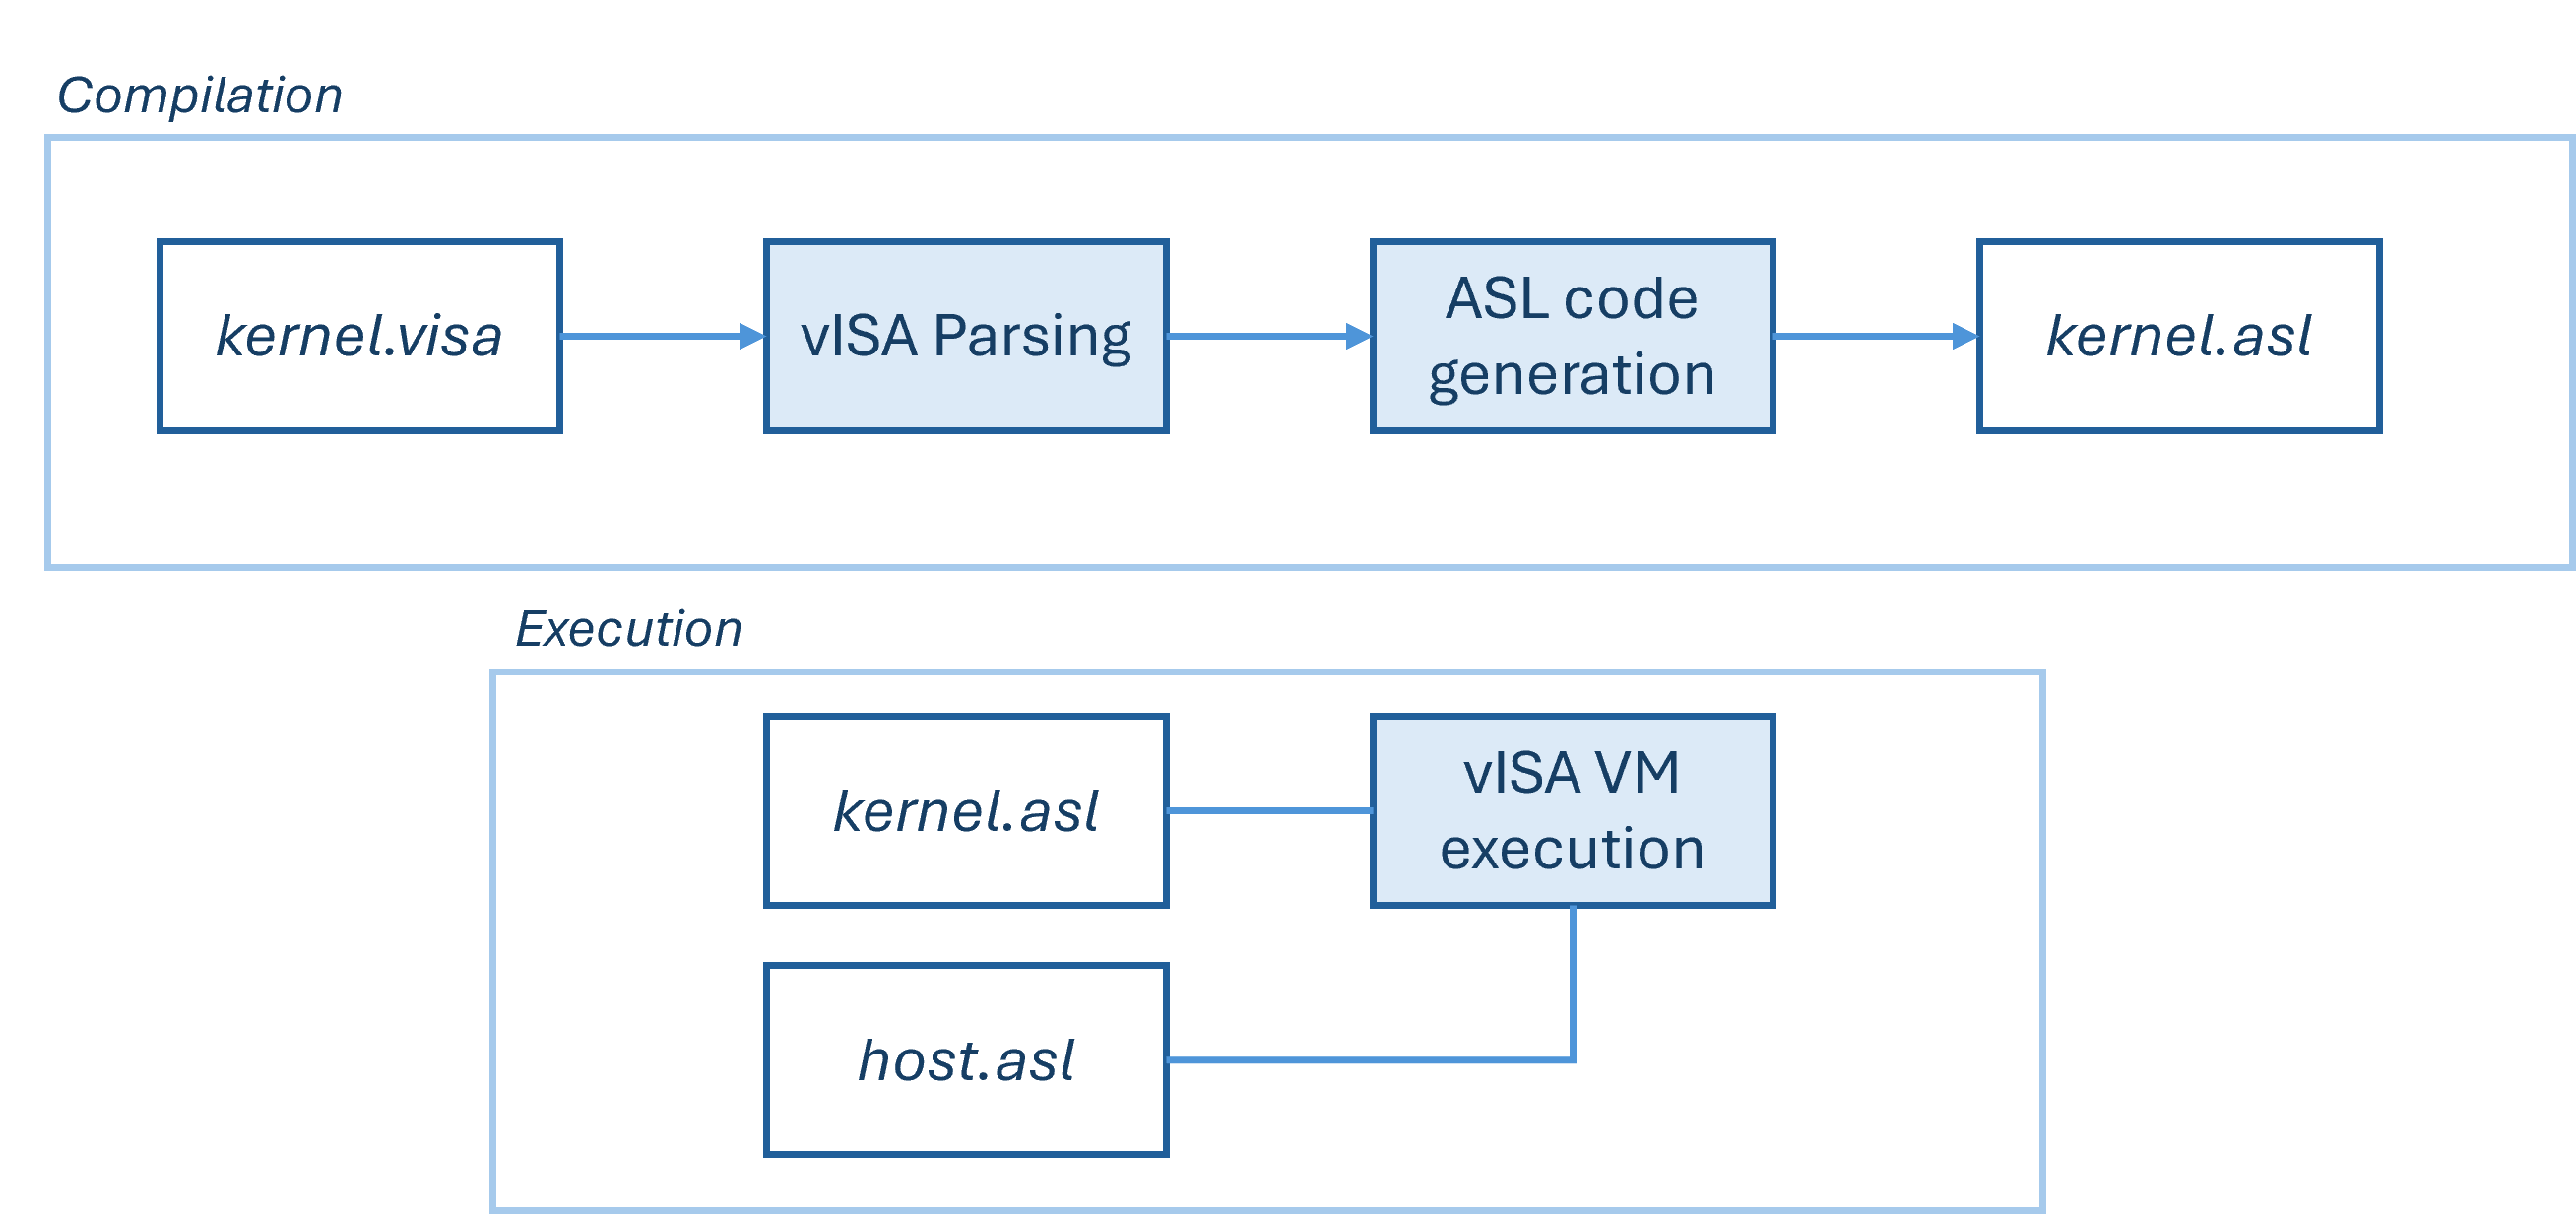
\includegraphics[width=0.8\textwidth]{img/workflow.png}
    \caption{Replace with VM diagram}
    \label{fig:workflow}
\end{figure}

The machine state contains all the globally defined variables that describe the
current state and configuration of the vISA virtual machine. It consists of
three main components: Data memory, which stores the values of registers and
variables following vISA's memory model. Instruction memory, which contains the
encoded program instructions that the virtual machine will execute. And the
control state, which contains auxiliary variables necessary to model the
behavior of the machine.

The machine behavior models all the procedures the machine can do. These are
program execution, memory operations and machine reset. Program execution is
done in steps, where each steps goes through three stages. Step execution
begins with the arbiter, responsible of choosing the next instruction to
execute and reactivates disabled threads. Then the fetch/decode stage retrieves
the instruction from instruction memory, decodes the opcode and operands and
invokes the corresponding operation. Finally the execution stage performs the
actual operation and writes back to memory. Memory operations modify data
memory and include variable allocation, reading and writing. Variable
allocation is used when loading workloads into the virtual machine, and
read/write operations are used during program execution. The machine reset
procedure returns GPU state to its initial configuration.

The translation tool takes vISA code and generates an equivalent ASL file to be
executed by the specification. A general workflow graph for running the
specification is shown on Figure \ref{fig:workflow}. The proposed and
implemented execution scheme has two parts: compilation and execution.


\begin{figure}[htbp]
    \centering
    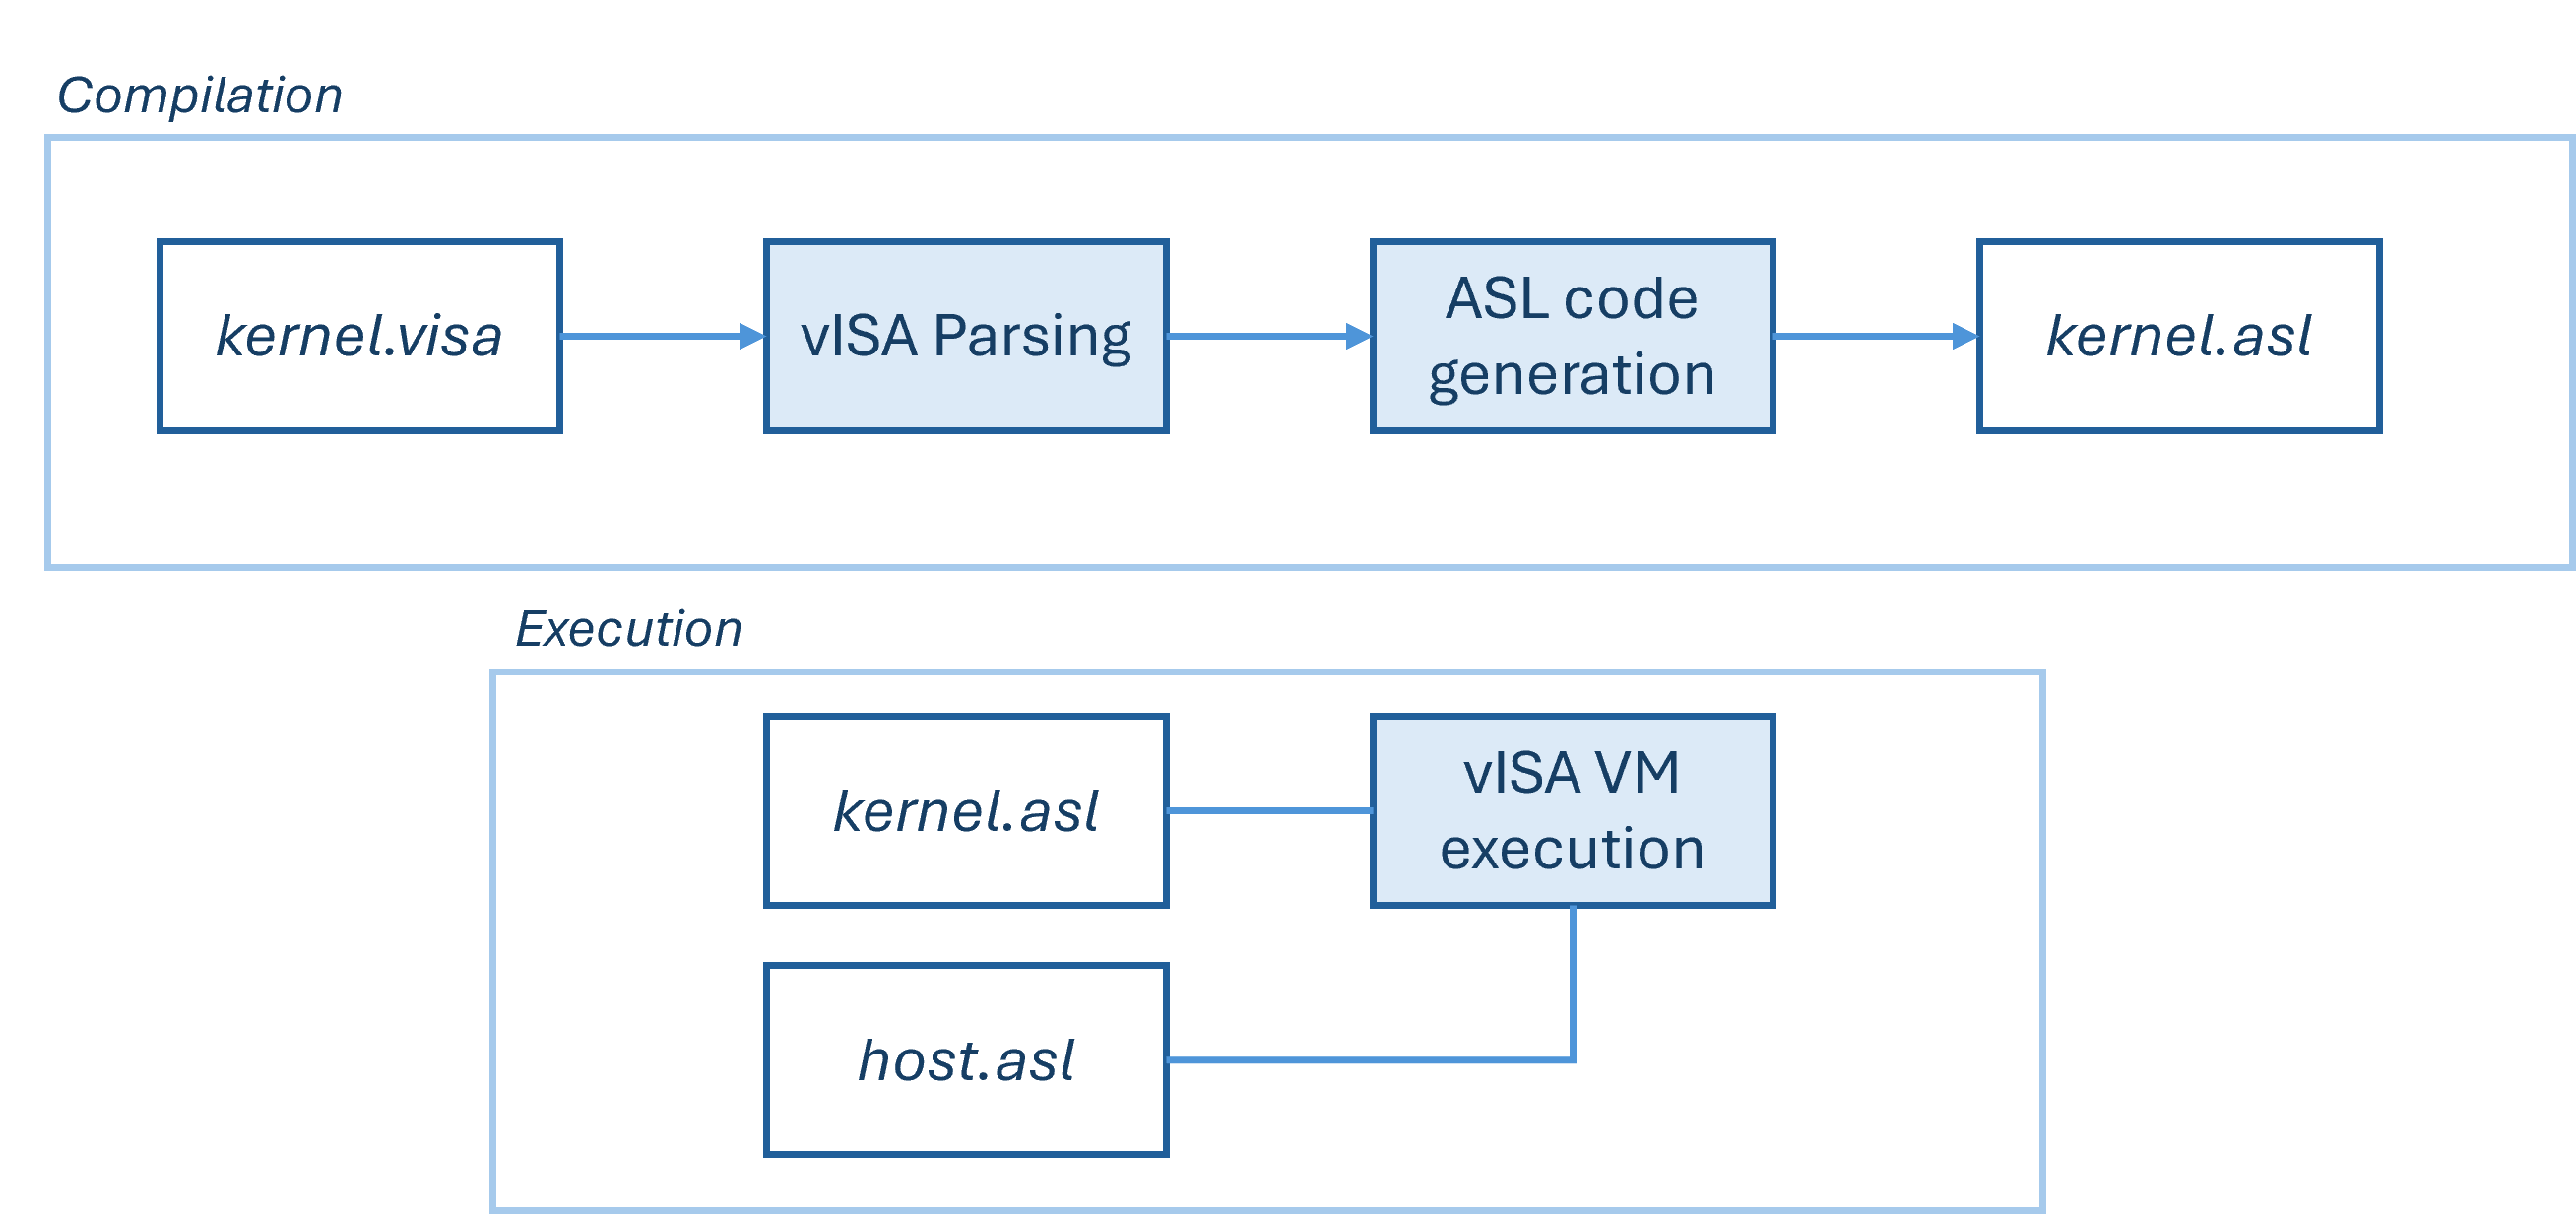
\includegraphics[width=0.8\textwidth]{img/workflow.png}
    \caption{Specification workflow}
    \label{fig:workflow}
\end{figure}

In the compilation part, we parse the vISA code with a lexical analyzer, and
load the code into an abstract syntax tree. Then, we generate a special ASL
file that loads instructions to the virtual machine, allocates registers and
variables to memory, and resolves labels and addresses. In the execution part
the generated ASL file is loaded into the vISA virtual machine, allowing the
instructions to be emulated in the ASL specification. An optional file for host
code can also be loaded to setup the data for the kernel parameters.

\section{Overview}
Here explain the context of the problem we face and how we overcome it,
problems coming from implementing a virtual ISA.

\section{Memory}
\section{Program representation}

\section{Machine State}

The machine state contains all the globally defined variables that define the
configuration and state of the vISA specification. The state is divided into
three components that we call data memory, instruction memory, and control
state.

Data memory models the memory spaces and hierarchy of vISA. Since vISA provides
a virtual memory model that allows an unlimited number of registers and
variables, we implement a dynamic memory allocation system to model vISA's
memory semantics within the restrictions of the ASL specification.

Each vISA memory space is represented as a bit array of predefined size, which
stores the data of their respective variables and registers.

Each memory space implements a linear allocation strategy. The machine state
maintains separate pointers for each memory space, tracking the next available
address for allocation. For thread-private spaces, allocation accounts for the
per-thread replication by multiplying the variable size by 32. For shared
spaces, variables are allocated once and shared across all threads.

We define a symbol table to map vISA variables and their declaration
information and memory address. Variable information is stored in an array of
variable records, where each record stores the variable's name, memory space,
address, bitwidth, and offset. When a variable is declared in a vISA kernel,
the allocation procedure determines the appropriate memory space, calculates
the next available address, and creates a new variable record in the table. The
retrieval of variable information is done through a linear search, matching by
the variables name. Label information is also stored in a separate symbol
table, mapping the label's name to its address in instruction memory. This
allows the virtual machine to access labels addresses during runtime.

Read and write operations use the symbol table to fetch the memory locations of
vISA variables. For private variables, where each thread saves a different
value, address calculation is done by combining the base address with the
thread specific offset. Bit-slice operations are then applied to extract or
update the appropriate portion of the memory space bit arrays.

On the other hand, instruction memory contains the instructions that the
virtual machine will execute. It is implemented as an array of Instruction
records, where each record contains all the information necessary for the
virtual machine to dispatch and execute the instructions. Some of the record's
fields are the instruction's opcode, source and destination operands, and
qualifiers. With this approach, instructions don't need to be explicitly
decoded. Data and instruction memory are initialized by the translation tool,
as a result of parsing the input vISA code.

Finally, the control state contains all the control and auxiliary variables
necessary to configure the virtual machine and handle execution. The most
relevant are: the program counter, an integer that indicates the address of the
instruction being executed by the virtual machine, its value corresponds to the
index of the instruction of the instruction memory array. The execution mask, a
32 bit array that indicates the active threads for the current execution step,
a value of '1' for the Nth bit means that the Nth thread is active, while '0'
means its inactive. The thread program counter is an array of 32 integers, that
tracks the program counter for each thread in the subgroup.

\section{Program Execution}

The main procedure of the virtual machine is program execution. This is done in
architectural steps, where instructions are fetched, executed and the machine
state is modified. This is done until all threads have finished execution. Each
step the virtual machine, chooses which

\section{vISA Parser}

To analyze vISA code, we must first parse the plain-text assembly language
instructions according to the instruction set specification presented in
Chapter X. Our parser converts input vISA code into an abstract syntax tree
(AST) that captures the main program structure using a standard parsing
toolchain for OCaml. OCamllex for lexical analysis and Menhir for parsing.

We present a context-free grammar for vISA, that will be the base of the
parser. As shown in Listing X, the grammar specifies that a vISA kernel
consists of a kernel declaration followed by zero or more variable declarations
and zero or more statements, where statements can be either instructions or
labels. The grammar uses standard BNF notation where \lstinline{<exp>*} denotes
zero or more repetitions of expression \lstinline{exp}, and includes regular
expressions for terminal symbols such as identifiers and immediate values.

\begin{center}
\begin{lstlisting}[numbers=none]

<kernel>      ::= <kernel_dec> <declaration>* <statement>*
<statements>  ::= <statement>
                | <statement> <statements>
<statement>   ::= <instruction> ";"
                | <label> ":"
<instruction> ::= <opcode> <qualifier>* <operands>
                | <opcode> <qualifier>*
                | <opcode> <operands>
                | <opcode>
<qualifier>   ::= <bitwidth>
                | <space>
                | <condition>
                | ...
<kernel_dec>  ::= ".kernel" <variable> "(" <parameters> ")"
<parameter>   ::= ".param[" <number> "]" <identifier>
<parameters>  ::= <parameter>
                | <parameter> "," <parameters>
<declaration> ::= ".pred" <identifier>* ";"
                | <space> <vsize> <bitwidth> <identifier>* ";"
                | <space> <bitwidth> <identifier>* ";"
<space>       ::= ".reg" | ".private" | ".shared" | ".global" | ".const" | ".param" 
<vsize>       ::= ".v2" | ".v3" | ".v4"
<bitwidth>    ::= ".8b" | ".16b" | ".32b" | ".64b"
<condition>   ::= ".eq" | ".ne" | "gt" | "ge" | "lt" | "le"
<operands>    ::= <operand> "," <operand> "," <operand> "," <operand>
                | <operand> "," <operand> "," <operand> 
                | <operand> "," <operand>
                | <operand>
<operand>     ::= "[" <identifier> "]"
                | "[" <identifier> "+" <identifier> "]"
                | "[" <identifier> "+" <immediate> "]"
                | <identifier>
                | <immediate>
<identifier>  ::= "%" [a-zA-Z0-9_]*
<immediate>   ::= ['0'-'9']*
                | "-" ['0'-'9']*
                | "0x" ['0'-'9']*

\end{lstlisting}
\end{center}

OCamllex performs lexical analysis by scanning the input character stream and
recognizing individual tokens based on regular expressions that correspond to
the terminal symbols defined in our grammar. When a character sequence matches
a regular expression, OCamllex executes the associated OCaml code to produce a
token with its corresponding type and value. A result of the tokenization
process is shown in Table X using the instruction
\lstinline{ucmp.lt.32b %p1, %r6, 0xF;} as an example, where each element is
mapped to its appropriate token type.

\begin{center}
\begin{tabular}{ |c|c|c| } 
 \hline
 \textbf{string} & \textbf{token} \\ 
 \hline
 ucmp & OPCODE \\ 
 \hline
 .lt & QUALIFIER \\
 \hline
 .32b & BITWIDTH \\
 \hline
 \%p0 & PREDICATE \\
 \hline
 , & COMMA \\
 \hline
 \%r0 & REGISTER \\
 \hline
 , & COMMA \\
 \hline
 0xF & HEX\_INT \\
 \hline
 ; & SEMICOLLON \\
 \hline
\end{tabular}
\end{center}

Menhir, is a parser generator based on OCamlyacc. It processes the token stream
according to the production rules defined in the context-free grammar. For each
grammar production rule, there is an associated parser action that executes
when the rule is matched, transforming the input tokens into the structured AST
types shown in Listing X. In the AST, the \texttt{kernel} type represents a
complete vISA kernel, \texttt{instr} types represent individual instructions
and labels, and \texttt{operand} types cover the various operands supported by
vISA instructions, as shown in Chapter X.


\begin{lstlisting}
type operand =
    | Operand of string
    | NegOperand of string
    | LabelOperand of string
    | Imm of string
    | BinAddrOp of operand * operand
    | AddrOp of operand

type kerneldef =
    | Parameter of string * addrspace * int
    | NoParameter

type vardef =
    | Variable of addrspace * int * operand list
    | Vector of addrspace * int * int * operand list
    | Predicate of operand list
    
type instr = 
    | Instruction of opcode * addrspace list * qualifier list * bitwidth list * operand list
    | Label of string

type kernel = 
    | Kernel of kerneldef list * vardef list * instr list
\end{lstlisting}

\section{Code Generation}

The parsed kernel is stored as the kernel type of our AST. The main goal of
code generation is to translate the vISA AST into ASL code that can be run by
our specification. This ASL code will tell the specification which variables to
allocate in the memory model, and what instructions will be executed.

The ASL specification has custom functions to allocate vISA variables into its
memory model, so kernel parameters and variable declarations will be translated
to specific ASL functions.

For the case od instructions, in the ASL specifications, instructions are
stored as records, with all the fields necessary to fully represent any vISA
instructions. An array of instruction records called InstructionBuffer,
contains the all the instructions that the specification will execute, with the
index as the address for each instruction. The instruction buffer is
instantiated as full of empty instruction records. So in code generation, for
vISA instruction in the AST, its corresponding fields are set in the ASL
instruction record.

ASL instructions are generated in a single pass,

We define a separate AST that represents the final ASL kernel. The main
differences between the ast are that: variable declarations are explicit for a
single variable instead for a list, adn instruction field types have an int
representing the instruction address.

\begin{lstlisting}
type set_kernel_params =
  | SetArgument of string * int
  | NoArgument

type allocate_var = 
  | InitRegister of string * int
  | InitVector of  string * int * int
  | InitPrivate of  string * int
  | InitShared of  string * int
  | InitGlobal of  string * int
  | InitConst of  string * int
  | InitParam of  string * int
  | InitPred of string

type set_instruction_fields =
  | SetOpcode of int * opcode
  | SetBitwidth of int * int
  | SetDst of int * string
  | SetSrc0 of int * string
  | SetSrc1 of int * string
  | SetSrc2 of int * string
  | SetSrc3 of int * string
  | SetImm0 of int * string
  | SetImm1 of int * string
  | SetImm2 of int * string
  | SetImm3 of int * string
  | SetAddrDst of int * operand
  | SetAddrSrc of int * operand

type kernel = 
  | Kernel of set_kernel_params list * allocate_var list * set_instruction_fields list list

\end{lstlisting}

In the vISA AST, variables are stored in a list. In the fianl ASL ast they are
allocated individually. For this, in the comoile process we map them into ther
individual nodes.


\section{}


\chapter{Implementing the ASL specification}

This chapter details the ASL implementation of the vISA specification,
translating the architectural concepts presented in Chapter into an executable
ASL specification.

\section{Objectives of the specification}
Here explain that implementing a virtual isa in asl has some difficulties.
Mainly that visa instructions only exists in text format, so to be read by asl,
they need to be encoded to a format readable by asl. Normally asl can directly
read instructions encoded to binary, using the bit pattern matching. One
alternative is to create a binary encoding for each vISA instruction. But this
approach is not viable because we have an unlimited number of virtual registers
and encoding them is not an easy task.

The other alternative is to encode the instructions into an ASL structure, in
the form of a record. And represent registers and variables as strings, and
have a memory system capable of allocating, reading and writing the variables
using the names as keys.

The other obstacle is the scope of the specification. The ASL specification
will concentrate on the minimum parallel unit of the SIMT model which is the
subgroup. So instructions will only be executed by a maximum of 32 work-items.

The objective of the specification is to replicate the visa virtual machine
defined in chapter x in ASL with the restrictions previously mentioned before.
It has to emulate parallel execution of workitems between a workgroup and
support all instructions, specially subgroup communication sintructions, and
control flow instructions.



\section{Modeling GPU}
Explain how memory is


\section{Modeling memory}
The memory system implementation translates vISA's memory model into ASL data
structures and access functions. This section details the representation of
memory spaces, variable management, and memory access operations.

\subsection{Memory Space Representation}
Each vISA memory space is implemented as a global bitvector, they are accesible
throughout all kernel execution, and provide direct bit access and
manipulation. Listing~\ref{lst:memory_spaces} shows the memory space
declarations:

\begin{lstlisting}[caption={Memory Space Declarations}, label={lst:memory_spaces}]
    var RegisterSpace : bits(RegisterSize);
    var PrivateSpace : bits(PrivateSize);
    var SharedSpace : bits(SharedSize);
    var GlobalSpace : bits(GlobalSize);
    var ConstantSpace : bits(ConstantSize);
    var ParameterSpace : bits(ParameterSize);
\end{lstlisting}

\subsection{Variable Representation}
\label{subsec:variable_representation}

The ASL specification keeps track of the variable data through an environment
system. Each variable is represented by a record containing all information
necessary for memory access operations.

\subsubsection{Variable Information Structure}
Listing~\ref{lst:variable_definition} shows the variable representation and
environment structure:

\begin{lstlisting}[caption={Variable Definition and Environment}, label={lst:variable_definition}]
enumeration MemorySpace { 
    Register, Private, Shared, Global, Constant, Parameter, Predicate 
};

record Variable {
    name    : string;     // Variable identifier
    space   : MemorySpace; // Memory space location
    size    : integer;    // Size in bits
    address : integer;    // Starting address in memory space
    offset  : integer;    // Per-thread offset for private variables
};

var Variables : array[NumberOfVariables] of Variable;
var VariableCount : integer;

func CreateVariableEntry(name : string, space : MemorySpace, size : integer, address : integer, offset : integer)
begin
    // Create variable record
    let variable = Variable {
        name = name,
        space = space,
        address = address,
        size = size,
        offset = size
    };

    // Add to environment
    Variables[VariableCount] = variable;
    VariableCount = VariableCount + 1;
end

\end{lstlisting}

The \texttt{offset} field enables efficient per-thread access to private
variables by specifying the bit distance between consecutive thread data within
the same variable.

\subsubsection{Memory Management}
Memory allocation tracking requires maintaining free space counters for each
memory space. These counters track the next available address in each memory
space, enabling sequential allocation without fragmentation.

\begin{lstlisting}[caption={Memory Allocation State}, label={lst:memory_state}]
var FreeSpaceRegister  : integer;
var FreeSpacePrivate   : integer;
var FreeSpaceShared    : integer;
var FreeSpaceGlobal    : integer;
var FreeSpaceConstant  : integer;
var FreeSpaceParameter : integer;
\end{lstlisting}

\subsection{Variable Allocation}
\label{subsec:variable_allocation}

Variable allocation process translates vISA variable declarations into memory
space allocation and environment entries. The process handles both scalar and
vector variables with appropriate memory layout considerations.

\subsubsection{Scalar Variable Allocation}
The base allocation function handles memory space selection and environment management:

\begin{lstlisting}[caption={Scalar Variable Allocation}, label={lst:scalar_allocation}]
func AllocateVariable(name : string, size : integer, space : MemorySpace)
begin
    var address : integer;
    var allocation_size : integer;

    // Calculate allocation size based on memory space type
    case space of 
        when Register, Private =>
            allocation_size = size * 32;  // Per-thread allocation
            address = GetFreeSpace(space);
            UpdateFreeSpace(space, allocation_size);
        when Shared, Global, Constant, Parameter =>
            allocation_size = size;       // Single allocation
            address = GetFreeSpace(space);
            UpdateFreeSpace(space, allocation_size);
    end

    CreateVariableEntry(name, space, size, address, offset);
end
\end{lstlisting}

\subsubsection{Vector Variable Allocation}
Vector variables require additional environment entries for swizzle access
patterns. For example, for a 2-element vector, the allocation creates 4
variable entries:

\begin{lstlisting}[caption={Vector Variable Swizzle Generation (v2 case)}, label={lst:vector_allocation}]
// Base vector allocation
let base_address = GetFreeSpace(Register);
let element_size = size;
let allocation_size = element_size * 2 * 32;  // 2 elements, 32 threads

UpdateFreeSpace(Register, allocation_size);

// Create swizzle variants
CreateVariableEntry(name,        base_address, element_size * 2);
CreateVariableEntry(name + ".x", base_address, element_size);
CreateVariableEntry(name + ".xy", base_address, element_size * 2);
CreateVariableEntry(name + ".y", base_address + element_size, element_size);
\end{lstlisting}

This approach allows direct access to vector and sub-vectors elements through
name-based lookup without the need of the specific swizzle address.

\subsection{Memory Access Operations}
\label{subsec:memory_access}

Memory access operations provide the interface between instruction execution
and the underlying memory system. All operations use a normalized 64-bit
interface to simplify instruction implementation.

\subsubsection{Variable Lookup}
Variable access begins with environment lookup to retrieve the variable information:

\begin{lstlisting}[caption={Variable Environment Lookup}, label={lst:variable_lookup}]
func GetVariableInfo(name : string) => Variable
begin
    for i = 0 to VariableCount - 1 do
        if Variables[i].name == name then
            return Variables[i];
        end
    end
    // Handle variable not found case
    assert FALSE;  // Variable must exist
end
\end{lstlisting}

\subsubsection{Memory Read Operations}
Read operations handle per-thread addressing for private variables and direct
access for shared and global variables:

\begin{lstlisting}[caption={Memory Read Implementation}, label={lst:memory_read}]
func ReadVariable(name : string, thread_id : integer) => bits(64)
begin
    let variable = GetVariableInfo(name);
    var result = Zeros(64);
    var effective_address : integer;

    // Calculate effective address
    case variable.space of
        when Register, Private =>
            effective_address = variable.address + (variable.offset * thread_id);
        when Shared, Global, Constant, Parameter =>
            effective_address = variable.address;
    end

    // Perform memory access
    case variable.space of
        when Register =>
            result[0 +: variable.size] = 
                RegisterSpace[effective_address +: variable.size];
        when Global =>
            result[0 +: variable.size] = 
                GlobalSpace[effective_address +: variable.size];
        // Additional cases for other memory spaces...
    end

    return result;
end
\end{lstlisting}

\subsubsection{Memory Write Operations}
Write operations are similar to read operation flow with value truncation to
match variable size:

\begin{lstlisting}[caption={Memory Write Implementation}, label={lst:memory_write}]
func WriteVariable(name : string, value : bits(64), thread_id : integer)
begin
    let variable = GetVariableInfo(name);
    let truncated_value = value[variable.size - 1 : 0];
    var effective_address : integer;

    // Calculate effective address (same logic as read)
    case variable.space of
        when Register, Private =>
            effective_address = variable.address + (variable.offset * thread_id);
        when Shared, Global, Constant, Parameter =>
            effective_address = variable.address;
    end

    // Perform memory write
    case variable.space of
        when Register =>
            RegisterSpace[effective_address +: variable.size] = truncated_value;
        when Global =>
            GlobalSpace[effective_address +: variable.size] = truncated_value;
        // Additional cases for other memory spaces...
    end
end
\end{lstlisting}

\subsection{Instruction buffer and encoding}
\label{subsec:instruction_buffer}

Beyond variable storage, the memory system must save kernel instructions to
enable runtime instruction access and control flow management. By maintaining
all kernel instructions in memory during execution, the specification gains
complete control over instruction sequencing, enabling accurate modeling of
complex operations such as jumps, branches, and divergent execution paths.

\subsubsection{Instruction Encoding Strategy}
\label{subsubsec:instruction_encoding}

vISA instructions lack a standardized binary representation, this presents an
opportunity to design an encoding optimized for ASL processing and human
readability. Rather than developing a complex binary encoding scheme, the
specification employs a record-based approach where each instruction field maps
directly to a record field.

The instruction encoding captures all information necessary for execution:
\begin{itemize}
    \item \textbf{Operation Identification:} Instruction opcode and execution semantics
    \item \textbf{Qualifiers:} Bit width specifications and operation modifiers
    \item \textbf{Operand Specification:} Destination and source operand identifiers
    \item \textbf{Operand Types:} Distinction between registers, immediates, and addresses
\end{itemize}

\subsubsection{Instruction Record}
\label{subsubsec:instruction_record}

The instruction record supports all vISA instruction variants through an
extensive field set. Listing~\ref{lst:instruction_record} shows the core
instruction structure:

\begin{lstlisting}[caption={Instruction Record Definition}, label={lst:instruction_record}]
enumeration Opcode { 
    add, sub, mul, // Arithmetic operations
    mov, sext,         // Movement and conversion
    load, store,          // Memory operations
    jump, ret,   // Control flow
    // Additional opcodes...
};

record Instruction {
    opcode     : OpCode;
    bitwidth   : integer { 8, 16, 32, 64 };
    
    // Destination operand
    dst        : string;
    
    // Source operands
    src0       : string;
    src1       : string;
    src2       : string;
    
    // Immediate operand flags and values
    src0_is_imm : boolean;
    src1_is_imm : boolean;
    src2_is_imm : boolean;
    imm0       : bits(64);
    imm1       : bits(64);
    imm2       : bits(64);
    
    // Address operand support
    src0_is_addr : boolean;
    src_addr     : AddressOperand;
    
    // Additional instruction-specific fields
    predicate    : string;
    negate_pred  : boolean;
    // ...
};
\end{lstlisting}

\subsubsection{Encoding Example}
\label{subsubsec:encoding_example}

Consider the vISA signed addition instruction template:

\begin{lstlisting}[caption={vISA Signed Addition Template}]
sadd.bitwidth dst, src0, src1
.bitwidth = {.16b, .32b, .64b}

Notes:
- dst must be a register
- src0, src1 must be a register or an immediate
\end{lstlisting}

A concrete vISA instruction \lstinline{add.32b %r1, %r0, 0xFFFF0000} translates
to the following record encoding:

\begin{lstlisting}[caption={Instruction Record Encoding Example}, label={lst:encoding_example}]
let add_example = Instruction {
    opcode      = add,
    bitwidth    = 32,
    dst         = "%r1",
    src0        = "%r0",
    src1        = "",           // Unused for immediate operand
    src0_is_imm = FALSE,
    src1_is_imm = TRUE,
    imm1        = 0xFFFF0000,
    // Remaining fields use default values
};
\end{lstlisting}

The encoding scheme distinguishes between operand types through auxiliary boolean fields:

\begin{description}
    \item[Register Operands:] Variable names stored in string fields
    (\lstinline{src0}, \lstinline{src1}, etc.)
    \item[Immediate Operands:] Values stored in dedicated immediate fields
    (\lstinline{imm0}, \lstinline{imm1}, etc.) with corresponding boolean flags
    (\lstinline{src0_is_imm}, \lstinline{src1_is_imm}, etc)
    \item[Address Operands:] Complex addressing modes stored in specialized
    address operand structures
\end{description}


\subsubsection{Instruction Buffer Implementation}
\label{subsubsec:instruction_buffer_impl}

The instruction buffer supports sequential storage for all kernel instructions,
providing free access during execution:

\begin{lstlisting}[caption={Instruction Buffer Declaration}, label={lst:instruction_buffer}]
var InstructionBuffer : array[MaxInstructions] of Instruction;
var InstructionCount : integer;
\end{lstlisting}

The buffer size is configurable to accommodate kernels of any size. The
\lstinline{InstructionCount} variable tracks the number of valid instructions
that have been loaded into the buffer.

\subsubsection{Instruction Loading and Access}
\label{subsubsec:instruction_access}

Instructions are loaded into the buffer during kernel initialization and
accessed via program counter indexing during execution:

\begin{lstlisting}[caption={Instruction Buffer Access Pattern}, label={lst:instruction_access}]
func LoadInstruction(instruction : Instruction, pc : integer)
begin
    assert pc < MaxInstructions;
    InstructionBuffer[pc] = instruction;
    if pc >= InstructionCount then
        InstructionCount = pc + 1;
    end
end

func FetchInstruction(pc : integer) => Instruction
begin
    assert pc >= 0 && pc < InstructionCount;
    return InstructionBuffer[pc];
end
\end{lstlisting}

\section{SIMT Execution Model Implementation}
\label{sec:simt_execution}
The ASL specification implements a step-based execution model that emulates
SIMT semantics. The model operates by reading from an initial instruction
buffer, memory state, and execution context, then executing discrete steps
until it reaches a terminal state. Each execution step follows a structured
pipeline that is able to handle uniform and divergent thread execution
patterns.

\subsection{GPU Execution State}
\label{subsec:gpu_state}
The GPU execution state encapsulates all information necessary to track the
current status of the virtual machine during each execution step. The state
keeps track of thread activity, instruction sequencing, and execution control
flow.

\begin{description}
    \item[Execution Mask:] A 32-bit array tracking active thread participation.
    When bit $n$ equals `0', thread $n$ is inactive and will not participate in
    the current instruction execution. When bit $n$ equals `1', the thread is
    active and will execute the current instruction. Initially, all threads are
    active, but control flow procedures can activate or deactivate threads
    throughout execution.

    \item[Execution Instruction Pointer:] An integer indicating the position of
    the next instruction to fetch from the instruction buffer. This pointer is
    initialized to zero and typically increments by one after each execution
    step, unless modified by control flow instructions.

    \item[Increment IP Flag:] A boolean controlling automatic instruction
    pointer advancement. When \lstinline{TRUE}, the execution instruction
    pointer increments at step completion. When \lstinline{FALSE}, the pointer
    has been explicitly modified by an instruction and should not be
    automatically incremented.

    \item[Thread Instruction Pointers:] A 32-element integer array tracking
    individual thread program counters. Under uniform execution, all thread
    pointers match the execution instruction pointer. During divergent
    execution, individual threads may have different instruction pointer
    values.

    \item[Thread Termination Status:] A 32-bit array indicating completion
    status for each thread. Initially all zeros, individual bits are set when
    threads execute return instructions. When all bits equal `1', the
    \lstinline{execution_end} flag is activated.

    \item[Execution End Flag:] A boolean indicating whether all threads have
    completed execution. When \lstinline{TRUE}, step execution terminates.
\end{description}

\begin{lstlisting}[caption={GPU Execution State Definition}, label={lst:gpu_state}]
record GPUState {
    execution_mask : bits(32);      // Active thread mask
    execution_ip   : integer;       // Current instruction pointer
    increment_ip   : boolean;       // IP increment control
    thread_ip      : array[32] of integer; // Per-thread IP values
    thread_end     : bits(32);      // Thread completion status
    execution_end  : boolean;       // Global execution completion
};
\end{lstlisting}

\subsection{SIMT Instruction Pipeline}
\label{subsec:simt_pipeline}

The SIMT execution model implements a simplified pipeline that processes
instructions while managing thread divergence and convergence. The pipeline
consists of three main stages: fetch, decode, and execute, with specialized
handling for different instruction categories.

\subsubsection{Instruction Fetch Stage}
Each execution step begins with termination checking and instruction fetch:

\begin{lstlisting}[caption={Instruction Fetch Implementation}, label={lst:instruction_fetch}]
func ExecuteStep()
begin
    // Check for execution completion
    if state.execution_end then
        return;  // End early
    end
    
    // Fetch current instruction
    let instruction = FetchInstruction(state.execution_ip);
    
    // Proceed to decode and execute
    DecodeAndExecute(instruction);

    // Advance IP if necesary
    if state.increment_ip then
        AdvanceInstructionPointer();
    end
    
    return;  // End step
end
\end{lstlisting}

\subsubsection{Instruction Decode}
The decode stage classifies instructions into categories that require different
execution approaches:

\begin{enumerate}
    \item \textbf{Label Instructions:} Pseudo-instructions marking jump
    targets, they don't execute an instruction, but reactivate threads that
    jumped to the label.
    \item \textbf{Control Flow Instructions:} Jumps, and return requiring
    special divergence handling.
    \item \textbf{Subgroup Instructions:} Shuffle and reduction instructions
    need access to all threads so they require special handling.
    \item \textbf{Vector Instructions:} Standard vector instructions executed per-thread
\end{enumerate}

\begin{lstlisting}[caption={Instruction Classification and Dispatch}, label={lst:instruction_dispatch}]
func DecodeAndExecute(instruction : Instruction)
begin
    case instruction.category of
        when Label =>
            // Labels check threads and reactivate if necessary
            ReactivateThreads()
            
        when ControlFlow =>
            // Control flow instructions handle divergence directly
            ExecuteControlFlowInstruction(instruction);

        when SubGroup =>
            // Control flow instructions handle divergence directly
            ExecuteSubGroupInstruction(instruction);
            
        otherwise =>
            // Standard vector instructions use SIMT execution
            ExecuteVectorInstruction(instruction);
    end
end
\end{lstlisting}


\subsection{SIMT Vector Instruction Execution}
\label{subsec:vector_execution}

Vector instructions execute across all active threads simultaneously, with each
thread processing its own operand values.

\subsubsection{Per-Thread Operand Decoding}
The execution model processes vector instructions by iterating over active
threads and decoding operands for each thread individually:

\begin{lstlisting}[caption={SIMT Vector Instruction Processing}, label={lst:vector_processing}]
func ExecuteVectorInstruction(instruction : Instruction)
begin
    let active_threads = state.execution_mask;
    var results : array[32] of bits(64);
    
    // Skip execution if no threads are active
    if active_threads == Zeros(32) then
        return;
    end
    
    // Execute instruction for each active thread
    for thread = 0 to 31 do
        if active_threads[thread] == '1' then
            // Decode operands for this thread
            let src0 = DecodeOperand(instruction, 0, thread);
            let src1 = DecodeOperand(instruction, 1, thread);
            let src2 = DecodeOperand(instruction, 2, thread);
            
            // Execute instruction for this thread
            results[thread] = ExecuteInstruction(thread, instruction, 
                                             src0, src1, src2);
        end
    end
    
    // Write results back to destination operands
    WriteResults(instruction, results, active_threads);
end
\end{lstlisting}

\subsubsection{Operand Decoding Logic}
Operand decoding handles the three operand types supported by vISA: registers,
immediates, and addresses:

\begin{lstlisting}[caption={Per-Thread Operand Decoding}, label={lst:operand_decoding}]
func DecodeOperand(instruction : Instruction, operand_index : integer, 
                   thread : integer) => bits(64)
begin
    var result : bits(64);
    
    case operand_index of
        when 0 =>  // Source operand 0
            if instruction.src0_is_imm then
                result = instruction.imm0;
            elsif instruction.src0_is_addr then
                result = CalculateAddress(instruction.src_addr, thread);
            else
                result = ReadVariable(instruction.src0, thread);
            end
            
        when 1 =>  // Source operand 1
            if instruction.src1_is_imm then
                result = instruction.imm1;
            else
                result = ReadVariable(instruction.src1, thread);
            end
            
        when 2 =>  // Source operand 2
            if instruction.src2_is_imm then
                result = instruction.imm2;
            else
                result = ReadVariable(instruction.src2, thread);
            end
    end
    
    return result;
end
\end{lstlisting}

% Add Calculate address


\subsubsection{Instruction Execution Dispatch}
Individual instruction execution is then dispatched based on opcode to the
appropriate ASL implementation function:

\begin{lstlisting}[caption={Instruction Execution Dispatch}, label={lst:execution_dispatch}]
func ExecuteOperation(thread : integer, instruction : Instruction, 
                     src0 : bits(64), src1 : bits(64), src2 : bits(64)) => bits(64)
begin
    var result = Zeros(64);
    
    case instruction.opcode of
        when add => 
            result = add(instruction.bitwidth, instruction, src0, src1);
        when ld => 
            result = load(instruction.bitwidth, instruction, src0);
        when st => 
            store(instruction.bitwidth, instruction, src0, src1);
        when ret => 
            ret(thread);
        // Additional instruction cases...
    end
    
    return result;
end
\end{lstlisting}

\subsubsection{Result Write}
\label{subsec:result_writeback}

After instruction execution, results are written back to destination operands
for active threads. The write-back process respects the execution mask so
inactive thread memory does not get overwritten:

\begin{lstlisting}[caption={Result Writeback Implementation}, label={lst:result_writeback}]
func WriteResults(instruction : Instruction, results : array[32] of bits(64), 
                  active_mask : bits(32))
begin
    for thread = 0 to 31 do
        if active_mask[thread] == '1' then
            if instruction.write_addr then
                // Memory write is handled during instruction execution
            else
                // Write to register destination
                WriteVariable(instruction.dst, results[thread], thread);
            end
        end
    end
end
\end{lstlisting}

%\section{Modeling GPU step execution}

%Our GPU model executes by steps. It reads from an initial Instruction Buffer, Memory and State, and executes steps until it reaches an end of execution State. Each step consists of a cycle of fetching, decoding and instruction execution , with some checks in between in order to modify the GPU State. Listing X shows our definition of the GPU State.

%\subsection{GPU State}
%The GPU State represents the current status of the virtual machine during each execution step. In the State we keep track of the status of the active threads, the instructions pointers and other variables that help describe the configuration of the virtual machine.

%\begin{itemize}
 %   \item Execution Mask: Is a bit array of size 32 that keeps track of the active threads. If the N-th bit of the execution mask is '0' it means the N-th thread of the subgroup is not active and will not execute the current instruction. If it is '1', it is active and will participate in instruction execution. At the beginning of execution, each thread is set to be active, so the execution mask is all ones. During execution, instructions and the gpu model can affect the execution mask, activating and deactivating threads as needed.

  %  \item Execution Instruction Pointer: Is an integer and keeps track of the position of the next instruction in the Instruction Buffer to be executed. At the beginning is set to point to the first instruction in the buffer and, by default, is incremented by one at the end of each execution step, unless specified by the 'Increment IP' field.

  %  \item Increment IP: Is a boolean field that keeps track if the execution ip needs to be incremented. If set to true, the execution ip will be incremented by one at the end of the execution step, if set to false, it has already been modified by an instruction and will not be incremented for the current execution step.

  %  \item Thread Instruction Pointer: Is an integer array of size 32. It keeps track of the next instruction to be executed by each thread. Default behavior is that the thread ips are equal to the execution ip. But control flow instructions can change the instruction pointer of specific threads.

  %  \item Thread End: Is a bit array of size 32 that keeps track if a thread has finished its execution. It begins with all bits set to '0', if a thread executes a 'return' instruction, its corresponding bit is set to '1'. If all bits are equal to '1', the field 'Execution End' is set to true and execution will stop in the next step.

  %  \item Execution end: Boolean field that keeps track if all thread have ended execution. If set to true, execution stepping stops.
%\end{itemize}

%\begin{lstlisting}
%    record GPUState
%    {
%        execution_mask : bits(32);
%        execution_ip  : integer;
%        increment_ip : boolean;
%        thread_ip : array[32] of integer;
%        thread_end : bits(32);
%        execution_end : boolean;
%    };
%\end{lstlisting}
%
%\subsection{Fetching and Decoding}
%At the start of every execution step, the first thing we do is check if we have reached the end of execution, if that is the case we return and the step execution ends, terminating the program. If not, we fetch the instruction to execute in the step.

%For fetching, we get the corresponding instruction from the instruction buffer indicated by the instruction pointer, as shown in Listing X:

%\begin{lstlisting}
%    let instruction = InstructionBuffer[State.execution_ip];
%\end{lstlisting}

%Then we decode the fetched instruction. On decoding, first we check the instruction type, from this we have three possible cases, if the instruction is a label, a jump or subgroup, or a normal vector instruction. In the first case we do nothing and continue step execution as the instruction has done nothing, this because we encode labels as instructions to keep track labels positions in the buffer for jump instructions, more of this in Section X. Jump and subgroup instructions behaviour needs to access other threads and directly change gpu State, so the decoding is exposed on the instruction itself, so it goes a much simpler general decoding stage and othe fields decoding is done and exposed in the instruction itself. If not any of these two cases, the instruction goes though the general decoding process which is as follows:

%For the general vector case, decoding and eventual execution is done per thread, meaning we iterate over the active threads of the step, decode the instruction operands for each one, and then each thread executes the instruction. We use an array of size thirty two to keep track of the result of each execution, which then will be written to the destination operand if the instruction requires so.

%Lets look at the operand decoding process, we initiate a mutable 64 bit vector 'src' for each source operand, if the operand is am immediate value, we load the imm field from the instruction record into 'src', if it is an address operand, we get the address operand from the instruction record, calculate the address, and store it into 'src', if not any of these cases, we read from the register field specifying the thread id to get the corresponding value from memory. We do this for the three source operands an instruction might have. If an instruction uses less operands, it will default to read from a non existing register, returning for that operand 0.

%\begin{lstlisting}
%    func DecodeVector(instruction : Instruction)
%    begin
%        let validthreads = State.execution_mask;
%        var result : array[32] of bits(64);
%        
%        if validthreads != Zeros(32) then
%            for thread = 0 to 31 do
%                if validthreads[thread] == '1' then
%                    var src0 : bits(64);
%                    if instruction.use_imm0 then
%                        src0 = instruction.imm0[0 +: 64];
%                    else 
%                        if instruction.read_addr then
%                            src0 = CalculateAddress(instruction.src_addr, thread);
%                        else
%                            src0 = Read(instruction.src0, thread);
%                        end
%                    end
%                    var src1 : bits(64);
%                    if instruction.use_imm1 then
%                        src1 = instruction.imm1[0 +: 64];
%                    else
%                        src1 = Read(instruction.src1, thread);
%                    end
%    
%                    var src2 : bits(64);
%                    if instruction.use_imm2 then
%                        src2 = instruction.imm2[0 +: 64];
%                    else
%                        src2 = Read(instruction.src2, thread);
%                    end
%                    result[thread] = ExecuteVectorInstruction(thread, instruction, src0, src1, src2);
%                end
%            end
%    
%            for wthread = 0 to 31 do
%                if validthreads[wthread] == '1' then
%                    if instruction.write_addr then
%                        // WriteToAdrres handled by st
%                    else
%                        Write(instruction.dst, result[wthread], wthread);
%                    end
%                end
%            end
%        end
%    end
%\end{lstlisting}
%
%The last step is executing the instruction, with the operands ready, we then check the opcode of the %instruction and call the corresponding asl function to execute the instruction under the decoded parameters. For this we have a switch case covering all instruction opcodes that can be executed.

%\begin{lstlisting}
 %   func ExecuteVectorInstruction(thread : integer, instruction : Instruction, src0_data : bits(64), src1_data : bits(64), src2_data : bits(64)) => bits(64)
%    begin
%        let opcode = instruction.opcode;
%        var result : bits(64);
%        case opcode of
%            when iadd => result = iadd(instruction.bitwidth, instruction, src0_data, src1_data);
%            when isub => result = isub(instruction.bitwidth, instruction, src0_data, src1_data);
%            when smul => result = smul(instruction.bitwidth, instruction, src0_data, src1_data);
%            when umad => result = umad(instruction.bitwidth, instruction, src0_data, src1_data, src2_data);
%            when mov => result = mov(instruction.bitwidth, instruction, src0_data);
%            when zext => result = zext(instruction.to_bitwidth, instruction.from_bitwidth, instruction, src0_data);
%            when sext => result = sext(instruction.to_bitwidth, instruction.from_bitwidth, instruction, src0_data);
 %           when trunc => result = trunc(instruction.to_bitwidth, instruction.from_bitwidth, instruction, src0_data);
%            when asr => result = asr(instruction.bitwidth, instruction, src0_data, src1_data);
%            when shl => result = shl(instruction.bitwidth, instruction, src0_data, src1_data);
%            when shr => result = shr(instruction.bitwidth, instruction, src0_data, src1_data);
%            when ucmp => result = ucmp(instruction.bitwidth, instruction, src0_data, src1_data);
%            when scmp => result = scmp(instruction.bitwidth, instruction, src0_data, src1_data);
%            when and => result = and(instruction.bitwidth, instruction, src0_data, src1_data);
%            when ld => result = ld(instruction.bitwidth, instruction, src0_data);
%            when st => 
%                st(instruction.bitwidth, instruction, src0_data, src1_data);
%                result = Zeros(64);
%            when ret => 
%                ret(thread);
%                result = Zeros(64);
%        end
%        return result;
%    end
%\end{lstlisting}




\subsection{ASL Instruction Implementation}

Translating vISA instructions into ASL implementations requires careful
preservation of instruction semantics while adapting to the ASL execution
model's constraints and conventions. For this, ASL instruction functions accept
standardized parameters including bit width sizes, operand values and the
instruction record to access non standard parameters as instruction specific
qualifiers. With this approach, most instructions can be adapted to the ASL
execution model.

\begin{lstlisting}[caption={Standard ASL Instruction Function Signature}, label={lst:standard_signature}]
func instruction_name(bitwidth : integer {8, 16, 32, 64},
                     instruction : Instruction,
                     src0 : bits(64),
                     src1 : bits(64),
                     src2 : bits(64)) => bits(64)
\end{lstlisting}
The 64-bit operand constraint eliminates type conflicts while maintaining
semantic correctness. Instructions then extract the relevant bit width from the
operand value and execute with their assigned bitwidth.

\begin{lstlisting}[caption={Bit Width Extraction Pattern}, label={lst:bit_extraction}]
// Extract operands at specified bit width
let operand0 = src0[0 +: bitwidth];
let operand1 = src1[0 +: bitwidth];

// Perform operation at native bit width
let result = operand0 OPERATION operand1;

// Package result in 64-bit container
var output  = Zeros(64);
output[0 +: bitwidth] = result;
return output;
\end{lstlisting}

For complex instructions requiring additional parameters, the can access them
directly through the instruction record, supporting specialized behaviors while
mantaining consistency:

\begin{lstlisting}[caption={Instruction Parameter Access Pattern}, label={lst:param_access}]
// Access instruction-specific qualifiers
let conversion_mode = instruction.conversion_mode;
let rounding_mode = instruction.rounding_mode;
let conditional_flag = instruction.conditional_flag;
\end{lstlisting}

\subsubsection{Implementation Example: Bitwise AND Instruction}
\label{subsubsec:and_implementation}

The bitwise AND instruction demonstrates the systematic translation from vISA
specification to ASL implementation, illustrating how architectural semantics
are preserved within the ASL execution framework.

\paragraph{vISA Specification}
The vISA bitwise AND instruction is specified as:

\begin{quote}
\textbf{Syntax:} \texttt{and.bitwidth dst, src0, src1}

\textbf{Bit Widths:} \texttt{.bitwidth} $\in$ \{\texttt{.16b}, \texttt{.32b},
\texttt{.64b}\}

\textbf{Semantics:} \texttt{dst = src0 \& src1}

\textbf{Constraints:} All operands must have matching bit widths
\end{quote}

\paragraph{ASL Implementation}
The corresponding ASL implementation preserves the instruction semantics while
conforming to the standardized execution model:

\begin{lstlisting}[caption={ASL Bitwise AND Implementation}, label={lst:and_asl_impl}]
func and(bitwidth : integer {16, 32, 64},
         instruction : Instruction,
         src0 : bits(64),
         src1 : bits(64)) => bits(64)
begin
    var result : bits(64) = Zeros(64);
    
    // Extract operands at specified bit width
    let operand0 = src0[0 +: bitwidth];
    let operand1 = src1[0 +: bitwidth];
    
    // Perform bitwise AND operation
    let and_result = operand0 AND operand1;
    
    // Package result in standardized container
    result[0 +: bitwidth] = and_result;
    
    return result;
end
\end{lstlisting}

\section{Handling divergency / Control Flow}


The ASL specification implements control flow support to model SIMT execution
patterns, including both uniform and divergent thread execution. This section
details the implementation of control flow instructions and the mechanisms used
to handle thread divergence and convergence.

\subsection{Control Flow Instructions Overview}
\label{subsec:control_flow_overview}

vISA provides two primary control flow instructions that affect sequential execution flow:

\subsubsection{Return Instruction}
The return instruction terminates individual thread execution, marking the
thread execution as completed:

\begin{lstlisting}[caption={Return Instruction Implementation}, label={lst:return_impl}]
func ret(thread : integer)
begin
    state.thread_end[thread] = '1';
    
    // Check if all threads have completed
    if state.thread_end == Ones(32) then
        state.execution_end = TRUE;
    end
end
\end{lstlisting}

\subsubsection{Jump Instructions}
Jump instructions provide both unconditional and conditional control transfer
capabilities:

\begin{lstlisting}[caption={Jump Instruction Syntax}]
jump label              // Unconditional jump
jump.cond pred, label   // Conditional jump based on predicate
\end{lstlisting}

The unconditional jump transfers control for all active threads to the
specified label, while the conditional variant performs predicated branching
based on per-thread predicate evaluation, introducing divergence into the
execution model.

\subsection{SIMT Divergence Model}
\label{subsec:divergence_model}

The specification implements a lockstep execution model where threads are
activated and deactivated to handle divergent control flow.

\subsubsection{Execution Flow with Divergence}
Figure~\ref{fig:divergence_execution} illustrates thread execution in the
presence of jump instructions. The execution demonstrates how threads diverge
at conditional branches and re-converge when reaching common instruction
points.

\begin{figure}[htbp]
    \centering
    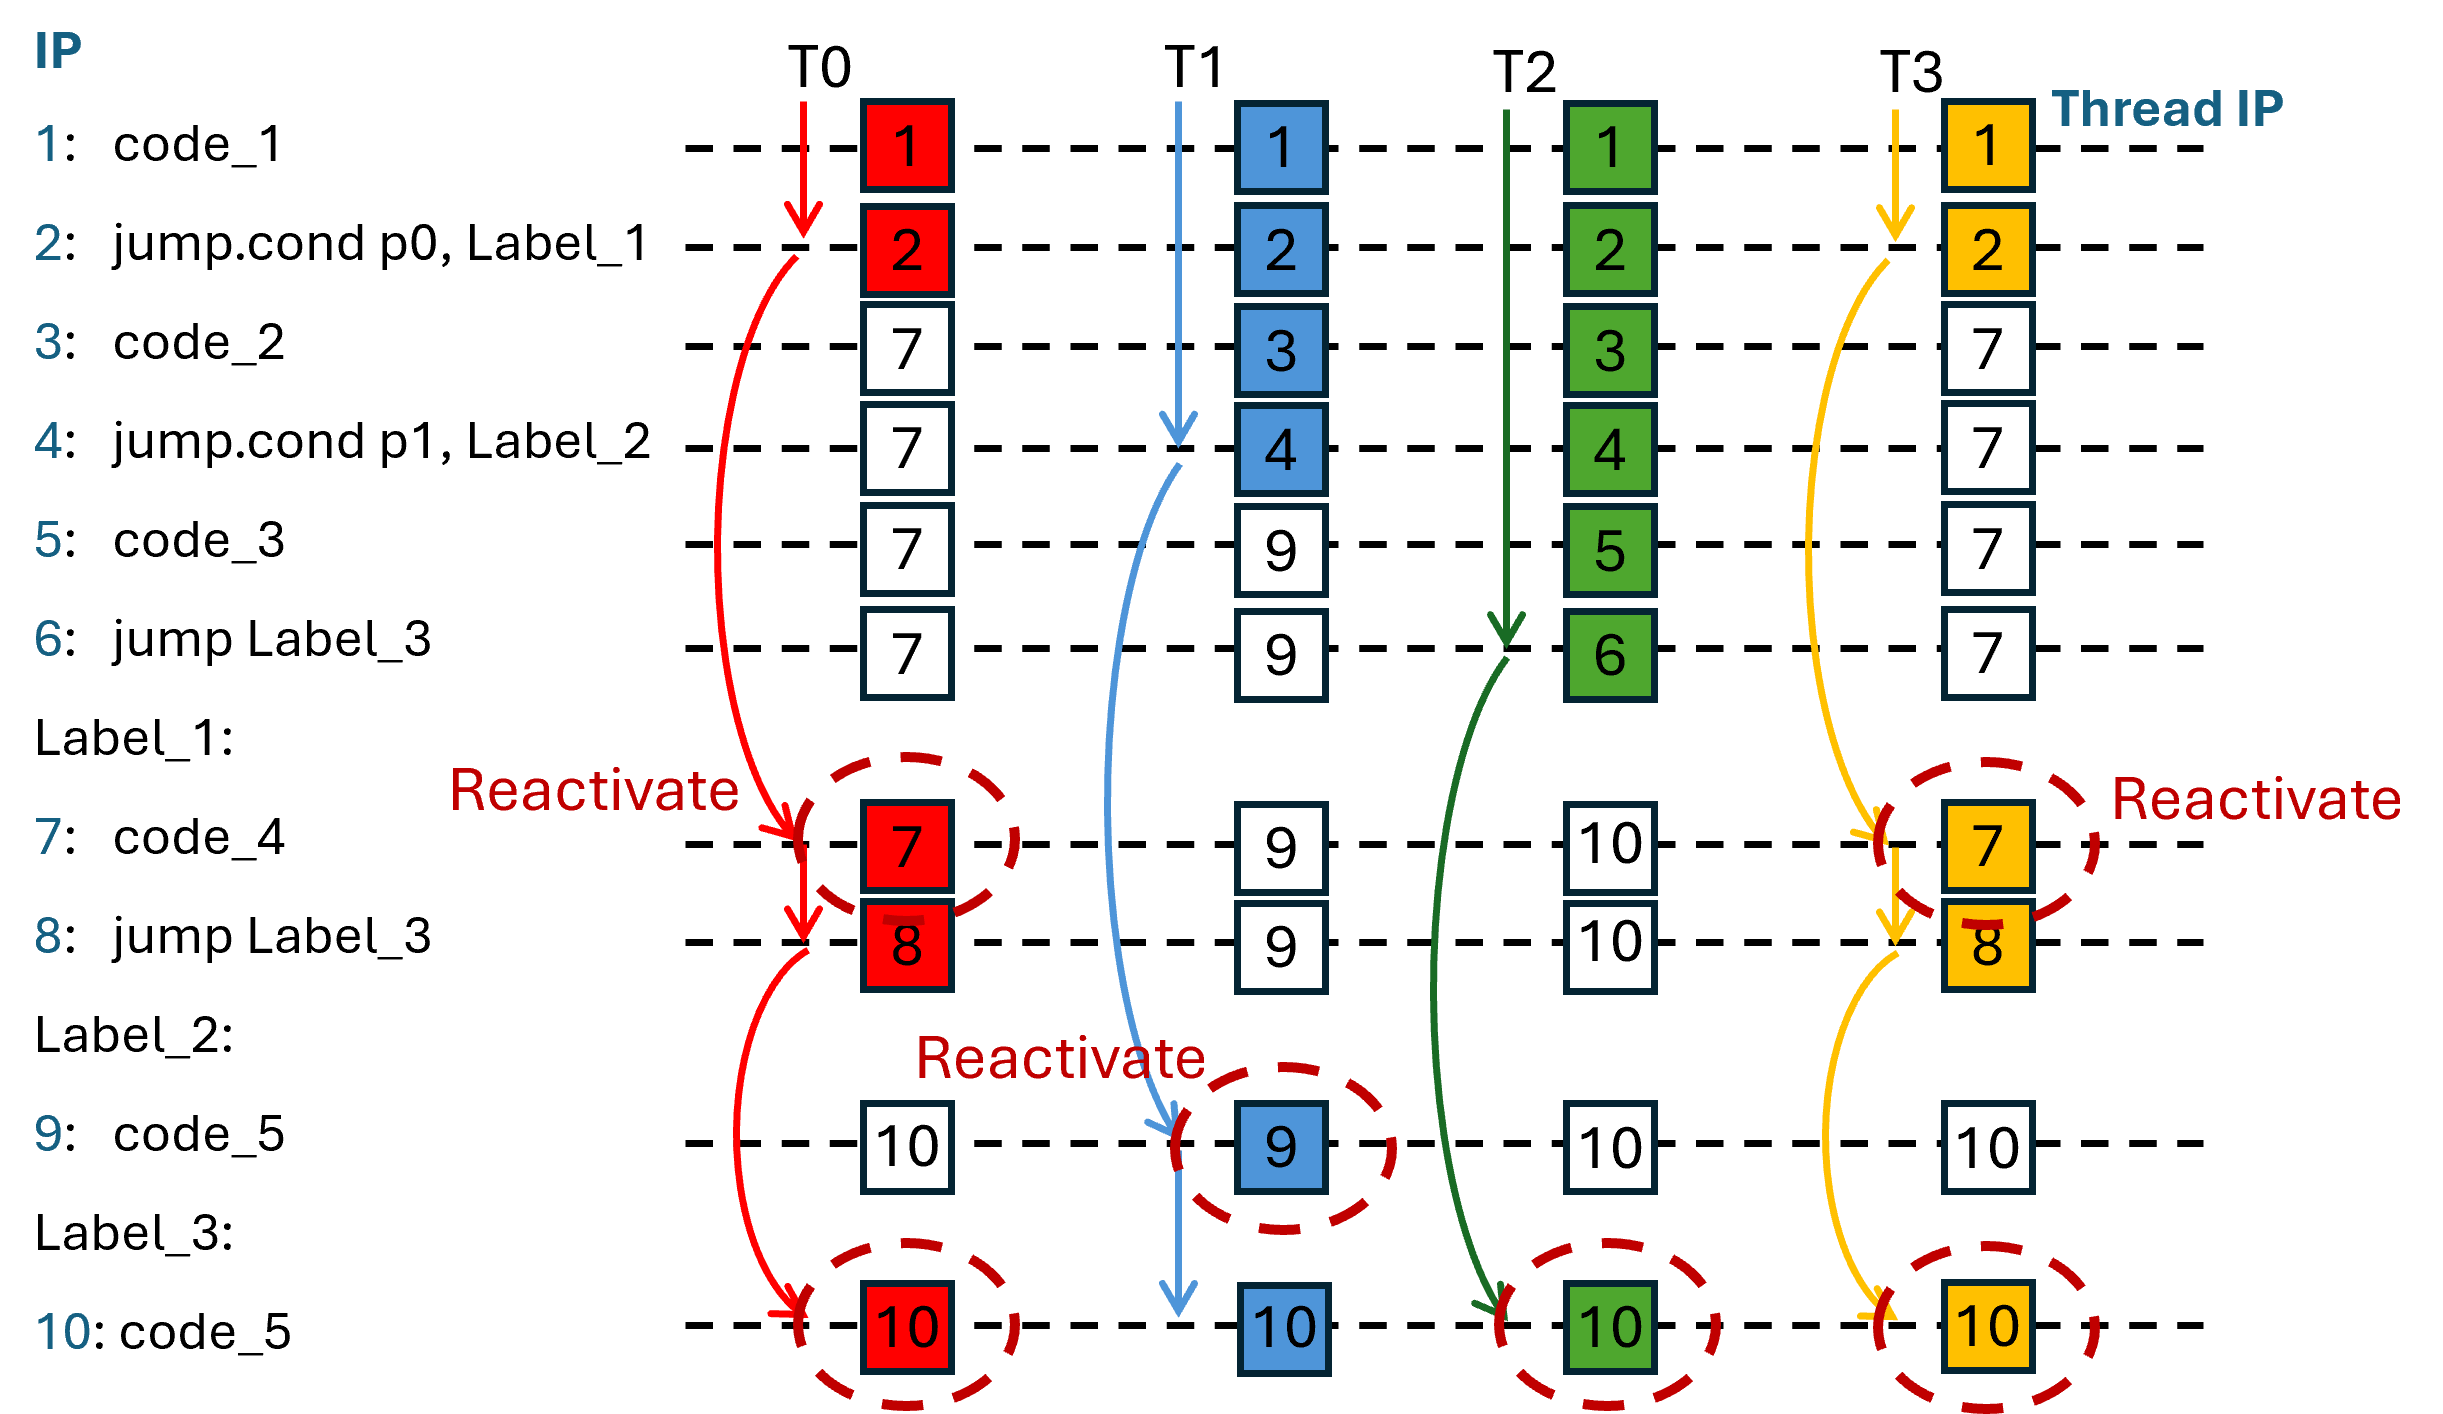
\includegraphics[width=0.8\textwidth]{img/jump3.png}
    \caption{Thread execution with divergency.}
    \label{fig:divergence_execution}
\end{figure}

At the left, the figure shows the instructions accompanied by their 'IP', where
jump instructions and labels are explicit, and general instructions that don't
affect execution flow are noted under a general name. To the right it shows the
execution of 4 threads, squares show the state of the thread in each execution
step, if it is colored, it means the thread is active, if not it is
deactivated, exemplifying the state of the execution mask. The numbers in each
square represent the each thread's IP.

Following the execution, at the start, all threads are active and execute
'code\_1' and increase their thread IP by one. Instruction 2 makes thread 0 and
3 jump to 'Label\_1', changing setting thread IP to 7 and deactivating them,
while the other threads continue normal execution. Then at instruction 4 thread
1 jumps to 'Label 2', it deactivates and sets its IP to 9. At instruction 7,
threads 0 and 4 are reactivated since they reached their target IP. Then at
instruction 8 they jump to 'Label\_3'. Instruction 9 reactivates thread 1 and
finally at instruction 10 all remaining threads are reactivated.

\subsubsection{Forward vs. Backward Jump Handling}
There are two possible cases for jumps, the case
Figure~\ref{fig:divergence_execution} shows only has forward jumps. Forward
jumps happen when the Label IP is greater than the IP of the jump instruction,
making the thread 'jump forwards' in execution. In this case the execution IP
increases by 1 and threads will be eventually reactivated when execution
reaches the label. The other case is backwards jump, this occurs when the Label
IP is less that the IP of the jump instruction, making the thread jump back in
execution. In this case execution IP can't be incremented, since execution will
never reach the label again and threads will not reactivate, so, instead of
increasing by one, threads that don't jump backwards are deactivated, and the
execution IP is set to the Label IP.

\begin{figure}[htbp]
    \centering
    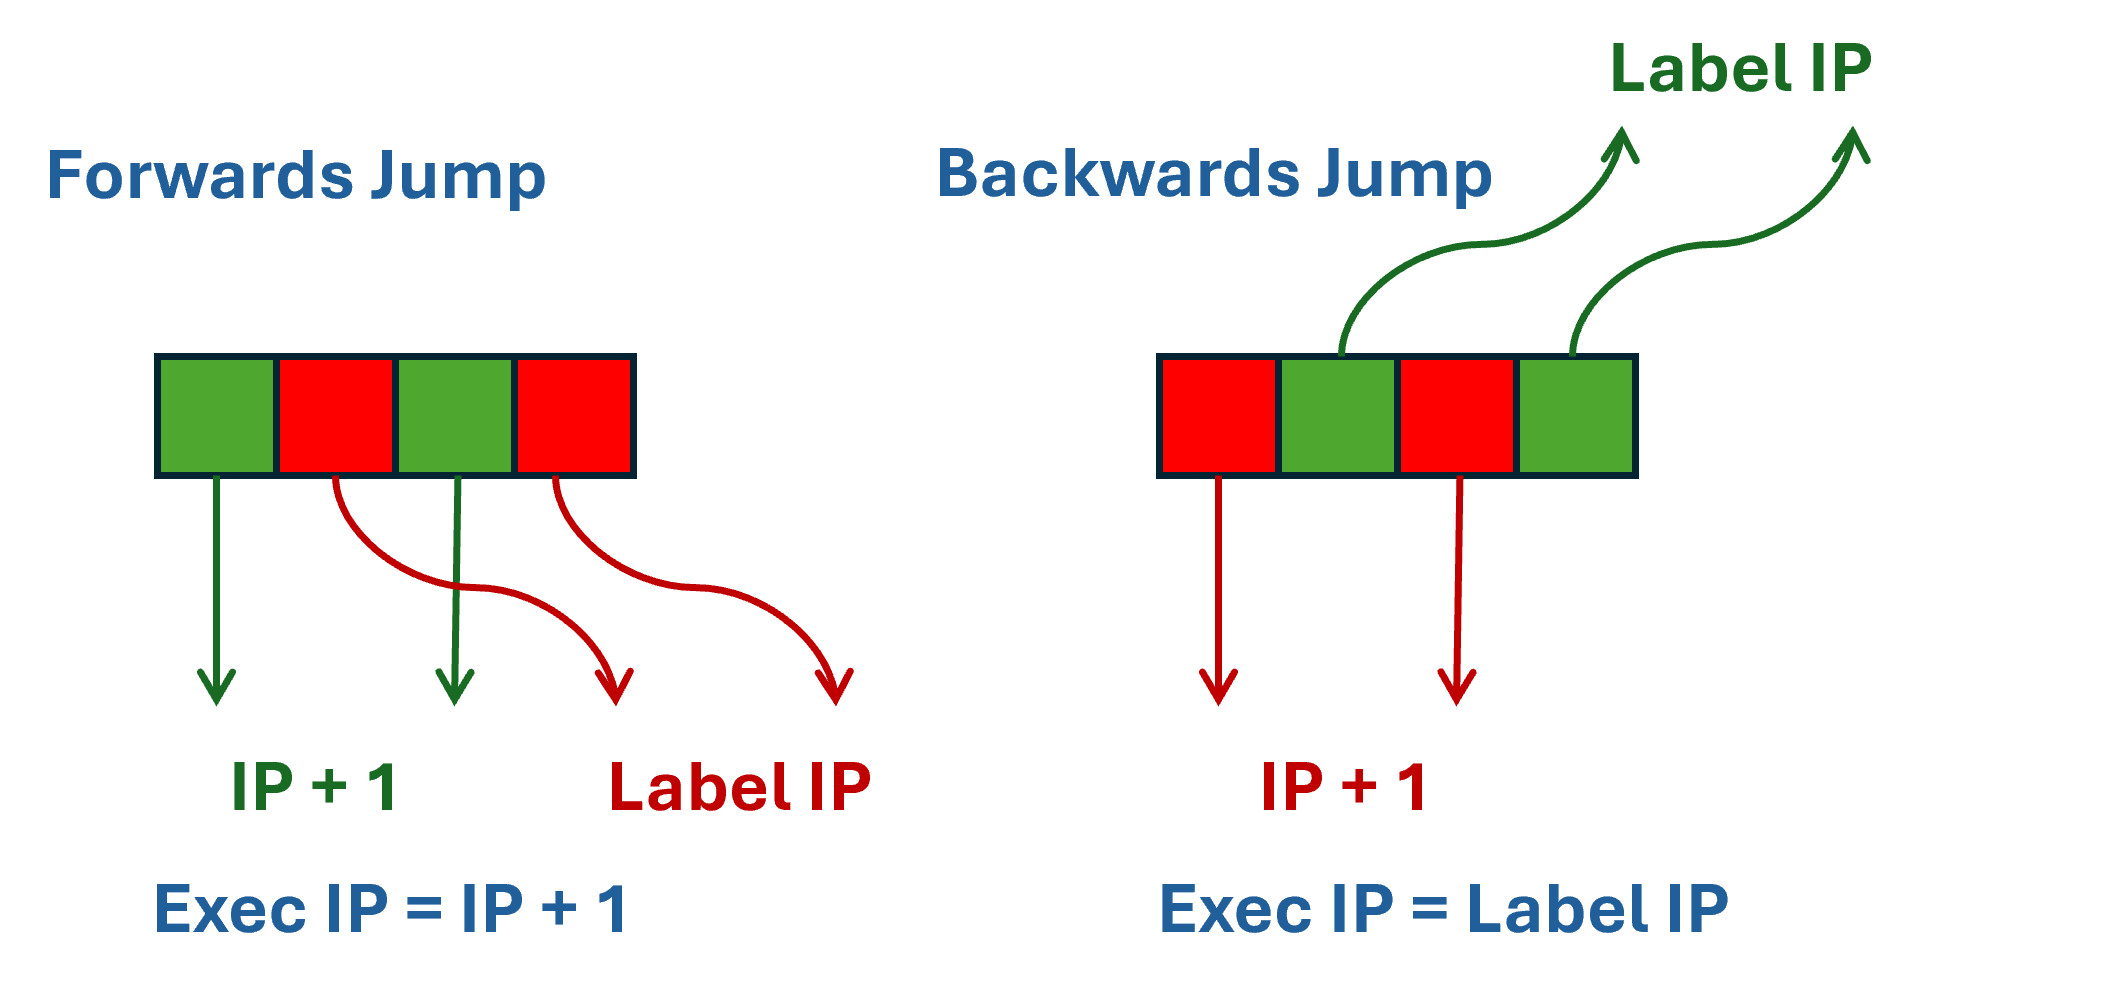
\includegraphics[width=0.8\textwidth]{img/jumpcases.png}
    \caption{Forwards and Backwards Jumps.}
    \label{fig:jump_cases}
\end{figure}


Figure~\ref{fig:jump_cases} illustrates the different strategies for forward
and backward jumps. In forwards jump, jumping threads are deactivated, noted by
red, their IP is set to the Label IP, and the execution IP is increased by 1.
For backwards jump, non-jumping threads are deactivated, and their IPs
increased by one, while jumping threads are kept activated, their IPs are set
to the Label IP and the execution IP is also set to the label IP.

\subsection{Keeping track of Labels}

To implement jump instruction in ASL, it is necessary to keep track the
position of the labels inside the instruction buffer. The approach is, through
an environment system, to associate each label name with their position in the
instruction buffer.

\begin{lstlisting}
    record Label {
        name : string;
        ip : integer;
    };

    var Labels : array[MaxLabels] of Label;
    var LabelCount : integer;
\end{lstlisting}

Labels are encoded as placeholder instructions within the instruction buffer
during kernel loading. By setting the label name to its corresponding program
counter, the specification is able to access each labels program counter during
jump instruction execution and correctly modify GPU state.

\begin{lstlisting}[caption={Label Instruction Encoding}, label={lst:label_encoding}]
// During kernel loading
InstructionBuffer[ip] = Instruction{ 
    opcode = label,
    label_name = label_name 
};
SetLabel(label_name, ip);
\end{lstlisting}



\subsection{Implementing jumps in ASL}
Unlike standard vector instructions, jump instructions cannot be executed
independently per thread due to their global state modification requirements.
So the thread for-loop execution is exposed as part of the instruction
behavior. This does not reflect how the GPU executes jumps, but it is necessary
to achieve the same result.

\begin{lstlisting}[caption={Jump Instruction Implementation}, label={lst:jump_implementation}]
    func jump(instruction : Instruction)
    begin
        let cond = instruction.goto_cond;
        let label_ip = GetLabelIp(instruction.label);
        var predicate : bit;
        var jumping_threads = Zeros(32);
    
        for thread = 0 to 31 do
            if state.execution_mask[thread] == '1' then
                if cond then // conditional jump
                    predicate = Read(instruction.dst, thread)[0];
                    if instruction.flip_pred then
                        predicate = NOT predicate;
                    end
                    if predicate == '1' then
                        state.thread_ip[thread] = label_ip;
                        jumping_threads[thread] = '1';
                    else
                        state.thread_ip[thread] = state.execution_ip + 1;
                    end
                else // normal jump
                    state.thread_ip[thread] = label_ip;
                    jumping_threads[thread] = '1';
                end
            end
        end
    
        let backwards_goto = label_ip < state.execution_ip;
    
        // all threads jump or theres backwards goto
        if backwards_goto && jumping_threads != Zeros(32) then
            state.execution_ip = label_ip;
            state.execution_mask = jumping_threads;
            
        else
            state.execution_mask = state.execution_mask AND (NOT jumping_threads);
            state.execution_ip =  state.execution_ip + 1;
        end
        increment_ip = FALSE;
    
    end
\end{lstlisting}

 Listing~\ref{lst:jump_implementation} shows the jump implementation. Jumping
 threads are recorded using a 32-bit mask. Conditional case handles predicate
 negation if necessary and threads that fulfill the condition are marked as
 jumping threads and their ip is updated to the label ip.


Then the corresponding jumping strategy is applied (forwards or backwards), by
comparing the label ip to the current execution ip. If at least one threads
does a backwards jump, the execution ip is set to the label ip, and the
execution mask is set to the jumping threads mask. In the forwards jump case,
jumping threads are deactivated in the execution mask and the execution ip is
incremented.


\begin{lstlisting}[caption={Thread Reactivation Logic}, label={lst:thread_reactivation}]
func CheckThreadReactivation()
begin
    for thread = 0 to 31 do
        if State.execution_mask[thread] == '0' && 
           State.thread_end[thread] == '0' &&
           State.thread_ip[thread] == State.execution_ip then
            // Reactivate thread that has reached its target
            State.execution_mask[thread] = '1';
        end
    end
end
\end{lstlisting}

\subsubsection{Thread Reactivation}
Thread reactivation occurs when the global execution instruction pointer
reaches positions where previously deactivated threads should resume execution,
this means labels are the reactivation points of the programs, as shown in
\ref{lst:instruction_dispatch}.

\begin{lstlisting}[caption={Thread Reactivation Logic}, label={lst:thread_reactivation}]
func ReactivateThreads()
begin
    for thread = 0 to 31 do
        if state.execution_mask[thread] == '0' && 
           state.thread_end[thread] == '0' &&
           state.thread_ip[thread] == state.execution_ip then
            // Reactivate thread that has reached its target
            state.execution_mask[thread] = '1';
        end
    end
end
\end{lstlisting}
\ref{lst:thread_reactivation} shows that if a deactivated thread still in
execution reaches their target label, it is reactivated.

\chapter{Testing framework}
In this chapter we cover the testing framework and test suite developed for the
vISA ASL specification. We present the vISA to ASL translation tool that
autotomizes the process of generating equivalent ASL code from vISA kernels
that are able to be run by the specification presented in X.x. We then present
the testing script responsible of executiong the ASL kernels and validating the
results. Finally we present the test suite generated to validate our
specification.


\section{Translation Tool}
To validate the ASL specification against real vISA code, we developed a simple
translation tool that converts vISA kernels into executable ASL code. The tool
allows for a structured approach to test the specification, by eliminating the
need for manual translation, which would be time-consuming and prone to error
by the target user. The tool is developed in OCaml, using Ocamllex for lexical
analysis and Menhir for parsing. The tool is limited to strictly translating
the kernels, it does not work as a host device and does not set up kernel host
code and parameter values. Kernels that do not have parameters and have a
single group of 32 threads can be executed directly after translation. If they

In listing X we take a look at a small vISA kernel that has divergent
execution. The kernel takes different paths based on the work-items's local id
of the work item. If \lstinline{localid % 4 == 0} it calculates the id value
decreased in 1, else it doubles it.

\begin{lstlisting}
.kernel  @test()
{
    .reg .32b %r0, %r1, %r2;
	.pred %p0;
    
	and.32b 	%r0, %localid.x, 3;
	ucmp.ne.32b 	%p0, %r0, 0;
	goto.cond !%p0, LBB0_1;
	iadd.32b 	%r1, %localid.x, -1;
	goto LBB0_3;
LBB0_1:                                
	iadd.32b 	%r1, %localid.x, %localid.x;
LBB0_3:                                 
	mov.32b	 %r2, %r1;
	return;
}
\end{lstlisting}

The tool is able to translate the kernel into ASL code that sets up the kernel
to be run in our specification. The tool handles kernel initialization using
standard predefined procedures, it resets the GPU state, defines the kernel
grid size, and initializes the special registers. It detects register
allocation and generates the corresponding ASL functions to initialize them in
memory. ost importantly, it encodes each instruction in order to the
instruction buffer, specifying all the necessary information to execute the
instruction. For labels, it both encodes them into the buffer and saves their
position in the label environment, allowing to perform jumps to their exact
position in runtime.

\begin{lstlisting}
// Kernel setup
Reset();
SetupKernel(32, 1);
SetupSpecialRegisters();

// Register allocation
Register("%r0", 32);
Register("%r1", 32);
Register("%r2", 32);
Pred("%p0");

// Buffer encoding
InstructionBuffer[0].opcode = and;
InstructionBuffer[0].inst_type = BitwiseInst;
InstructionBuffer[0].bitwidth = 32;
InstructionBuffer[0].dst = "%r0";
InstructionBuffer[0].src0 = "%localid.x";
InstructionBuffer[0].use_imm1 = TRUE;
InstructionBuffer[0].imm1 = 3;
...
// Label encoding
SetLabel("LBB0_1", 5);
InstructionBuffer[5].opcode = label;
InstructionBuffer[5].label = "LBB0_1"; 
\end{lstlisting}

The tools architecture follows a standard compiler pipeline. The lexer
tokenizes the input vISA code based on the terminal symbols defined in vISA
grammar. The parser then constructs an abstract syntax tree representing the
vISA kernel structure. The vISA AST is then transversed and transformed into
the target ASL specification AST. Finally, the ASL code is produced by printing
the instructions based on the ASL AST.

\subsection{Context Free Grammar of vISA}

Context free grammar of vISA is shown in listing X, in which \lstinline{<exp>*}
denotes that an \lstinline{exp} repeats zero or more times, and also include
regex expressions to note string and number symbols.
\begin{center}
\begin{lstlisting}[numbers=none]

<kernel>      ::= <kernel_dec> <declaration>* <statement>*
<statements>  ::= <statement>
                | <statement> <statements>
<statement>   ::= <instruction> ";"
                | <label> ":"
<instruction> ::= <opcode> <qualifier>* <operands>
                | <opcode> <qualifier>*
                | <opcode> <operands>
                | <opcode>
<qualifier>   ::= <bitwidth>
                | <space>
                | <condition>
                | ...
<kernel_dec>  ::= ".kernel" <variable> "(" <parameters> ")"
<parameter>   ::= ".param[" <number> "]" <identifier>
<parameters>  ::= <parameter>
                | <parameter> "," <parameters>
<declaration> ::= ".pred" <identifier>* ";"
                | <space> <vsize> <bitwidth> <identifier>* ";"
                | <space> <bitwidth> <identifier>* ";"
<space>       ::= ".reg" | ".private" | ".shared" | ".global" | ".const" | ".param" 
<vsize>       ::= ".v2" | ".v3" | ".v4"
<bitwidth>    ::= ".8b" | ".16b" | ".32b" | ".64b"
<condition>   ::= ".eq" | ".ne" | "gt" | "ge" | "lt" | "le"
<operands>    ::= <operand> "," <operand> "," <operand> "," <operand>
                | <operand> "," <operand> "," <operand> 
                | <operand> "," <operand>
                | <operand>
<operand>     ::= "[" <identifier> "]"
                | "[" <identifier> "+" <identifier> "]"
                | "[" <identifier> "+" <immediate> "]"
                | <identifier>
                | <immediate>
<identifier>  ::= "%" [a-zA-Z0-9_]*
<immediate>   ::= ['0'-'9']*
                | "-" ['0'-'9']*
                | "0x" ['0'-'9']*

\end{lstlisting}
\end{center}

\subsection{Abstract Syntax Tree of vISA}
Listing X shows the main types of the abstract syntax tree based of the vISA
grammar. In detail, the \texttt{prog} type corresponds to the top-level
\texttt{<kernel>} production, containing kernel parameter definitions, variable
declarations, and instructions that make the kernel. The operand type captures
all the possible operands an instruction can take, comprising of registers,
immediate, addresses and labels. The \texttt{vardef} type maps the different
variable definitions in a kernel, being regular declarations for registers or
variables, and vectors or predicates. Kernel arguments are separated from
regular variable definitions and are represented by the \texttt{kerneldef}
type. The kernel instructions are represented by the \texttt{instr} type which
captures opcodes, qualifiers and operands. Address spaces and bitwidths are
noted different as qualifiers in this type, since they are used in other
expressions and are parsed into their own types.

\begin{lstlisting}
type operand =
    | Operand of string
    | NegOperand of string
    | LabelOperand of string
    | Imm of string
    | BinAddrOp of operand * operand
    | AddrOp of operand

type kerneldef =
    | Parameter of string * addrspace * int
    | NoParameter

type vardef =
    | Variable of addrspace * int * operand list
    | Vector of addrspace * int * int * operand list
    | Predicate of operand list
    
type instr = 
    | Instruction of opcode * addrspace list * qualifier list * bitwidth list * operand list
    | Label of string

type prog = 
    | Program of kerneldef list * vardef list * instr list
\end{lstlisting}

\subsection{Abstract Syntax Tree of ASL spec}
Listing X shows the AST for the final ASL specification code. On translation we
map each node of the vISA AST to an ASL node, representing the final ASL code
to be printed. Types \texttt{set\_kernel\_params} and \texttt{allocate\_var}
are straightforward and map variable declarations to their corresponding ASL
functions for initialization in memory, keeping track of the name and size.
Instructions are translated into a list of type
\texttt{set\_instruction\_fields}, which represent encoding the information of
the instruction into the instruction buffer. Each node of this type has an
extra \texttt{int} field, which is used to keep track of the index of the
instruction buffer it is intended to be encoded to. All these types are
encapsuled into the \texttt{kernel} type, that represents the final ASL kernel.
\begin{lstlisting}
type set_kernel_params =
  | SetArgument of string * int
  | NoArgument

type allocate_var = 
  | InitRegister of string * int
  | InitVector of  string * int * int
  | InitPrivate of  string * int
  | InitShared of  string * int
  | InitGlobal of  string * int
  | InitConst of  string * int
  | InitParam of  string * int
  | InitPred of string

type set_instruction_fields =
  | SetOpcode of int * opcode
  | SetDst of int * string
  | SetSrc0 of int * string
  | SetLabel of int * string
  ...
type kernel = 
  | Kernel of set_kernel_params list * allocate_var list * set_instruction_fields list list
\end{lstlisting}

In summary, in this section we presented the vISA-ASL translation tool, that
takes vISA kernel source code, performs lexical analysis and parsing based on
our vISA context-free grammar to produce a vISA Abstract Syntax Tree, then
transforms this AST into an equivalent ASL specification AST, and generates
executable ASL code. This tool enables automated validation of our
specification against real GPU programs and provides a practical bridge for
developers to test existing vISA kernels within our ASL framework without much
manual translation effort.

\section{Test suite}
To test the specification, we developed a set of smoke tests. We build to test
the correctness of the behaviour of each instruction definition. Each vISA
instruction has its own test, where its behaviour is verified for all its
possible cases of qualifiers. We also include test divergent execution and
simple gpu workloads.

A smoke test consists of the vISA code we want to test, and the 'golden'
reference result, which are the expected values of the registers that contain
the results. We use a python script that builds and runs all the smoke tests.
The script records the vISA code and the expected results, runs the translator
over the vISA code, and appends a few lines of code to the genereated asl code,
it adds the ExecuteProgram function and the debug function printVar for each of
the result registers. Then the final asl code is executed, and the result
register values are compared to the expected ones, if there are differences,
the test fails. From each smoke test, five files are generated, the original
vISA code, the ASL code, the expected and actual results, and the execution
logs.

The reference results are calculated by hand. We provide a total of 15 tests.

